\documentclass[12pt,article,twosided]{memoir}
%% ::: Memoir class options for page size
%% ::: * the STOCK SIZE is LETTER
%% ::: * the TRIMMED SIZE is 6 x 9
\setlrmarginsandblock{1.25in}{*}{1}
\setulmarginsandblock{1.75in}{*}{1}
\setheadfoot{0.55in}{1in}
\checkandfixthelayout

\usepackage{polyglossia}
\setdefaultlanguage{english}
\setotherlanguage{sanskrit}
\setotherlanguage{tamil}
\setotherlanguage{telugu}
\setotherlanguage{kannada}
\setotherlanguage{malayalam}
\defaultfontfeatures{Mapping=tex-text}
\setmainfont[Numbers={Proportional},SmallCapsFont={TeX Gyre Termes},SmallCapsFeatures={Letters=SmallCaps,Numbers=Lining}]{IndUni-T}
\newfontfamily\tamilfont[Script=Tamil]{AksharUnicodeRegular}
\newfontfamily\sanskritfont[Script=Devanagari]{Jaini}
\newfontfamily\greekfont[Script=Greek]{GFS Porson}
\usepackage[shortcuts]{extdash}
\usepackage{tikz}
\usetikzlibrary{backgrounds, matrix, positioning, fadings, through}
\usepackage{pgf}
\usepackage{tipa}
\usepackage{amssymb}
\usepackage{fontawesome5}
\usepackage{totcount}
\usepackage{calc}
\usepackage{natbib}
	\bibpunct[: ]{(}{)}{; }{a}{ }{,}
\usepackage{xcolor}
\definecolor{Nesarlink}{HTML}{f6820b}
\definecolor{Nesarlinkdark}{HTML}{8a4b0b}
\definecolor{Nesarlinklight}{HTML}{fff0e0}
\usepackage{catchfile}
\usepackage{graphicx,graphbox}
\graphicspath{{images/}}
\usepackage{ragged2e}
\usepackage{tabularx}
\usepackage{changepage}
\usepackage{trimspaces}
\usepackage{framed}
\usepackage[most,breakable]{tcolorbox}
\usepackage[bottom,marginal,multiple]{footmisc}
\def\changemargin#1#2{\list{}{\rightmargin#2\leftmargin#1}\item[]}
\let\endchangemargin=\endlist 
\makeatletter
\renewcommand\@makefntext[1]{%
  \par \parindent=\z@ \noindent
  \llap{\@thefnmark.\quad}%
  {\addfontfeatures{Numbers=Lining}#1}%
}
\ExplSyntaxOn
\cs_set_nopar:Nn{\polyglossia@lang@frenchspacing:n}{\frenchspacing}
\ExplSyntaxOff
\CatchFileDef\slug{metadata/metadata-identifier.tex}{}
\CatchFileDef\doi{metadata/metadata-doi.tex}{}
\newcommand\Ndates{%
\IfFileExists{metadata/metadata-dates-submission.tex}{%
submitted \input{metadata/metadata-dates-submission.tex} {\fontspec{Noto Sans Math}⧫}}{}%
\IfFileExists{metadata/metadata-dates-acceptance.tex}{%
accepted \input{metadata/metadata-dates-acceptance.tex} {\fontspec{Noto Sans Math}⧫}}{}%
\IfFileExists{metadata/metadata-dates-publication.tex}{%
published December 8, 2024}{}
}
% TITLE COMMANDS:
% Ntitle produces Title (no subtitle)
\CatchFileDef\Ntitle{metadata/metadata-title.tex}{}
\title{\protect\trim{\Ntitle}}
% Ntitles produces Title: Subtitle
\newcommand{\Ntitles}{%
\IfFileExists{metadata/metadata-subtitle.tex}{%
{\trim{Meat Matters}}: Meat Matters}{%
Meat Matters}}
\CatchFileDef\citation{metadata/metadata-citation.tex}{}
\makeatother
\def\trim#1{\ignorespaces#1\unskip}
\newcommand{\Nyear}{\trim{2022}}
\newcommand{\Nauthor}{\trim{Jonathan Peterson}}
\author{\protect\Nauthor}
\newcommand{\article}{\trim{1}}
\newcommand{\iy}{\trim{1 (2024): 33–\total{page}.}}
\makeatother
\newcommand{\oldnums}[1]{{\fontspec[Numbers={Proportional,OldStyle}]{TeX Gyre TermesX}#1}}
\newcommand{\oldnumsbold}[1]{{\fontspec[Numbers={Proportional,OldStyle}]{TeX Gyre TermesX}\textbf{#1}}}
\setsecnumformat{\csname #1secnumformat\endcsname}
\newcommand\sectionsecnumformat{\oldnumsbold{\thesection}\quad }
\newcommand\onpage{\oldnums{\thepage}}
\newcommand{\bLozenge}{\mathbin{\blacklozenge}}

\regtotcounter{page}

% Button for CC 4.0 BY
\newcommand{\ccbylicenseButton}{%
\href{https://creativecommons.org/licenses/by/4.0/}{
\includegraphics[align=t,width=2cm]{byNesar.png}}}
% Link to journal
\newcommand{\journallink}{%
\expandafter\url\expandafter{https://nesarjournal.org/articles/\expandafter\slug}}
% Link to DOI
\newcommand{\doilink}{%
DOI: \expandafter\href\expandafter{https://doi.org/\expandafter\doi}{\doi}}
% Issue.Article (Year)
%\newcommand{\iay}{%
%\fontspec[Numbers={Proportional,OldStyle}]{TeX Gyre TermesX}issue \issue, article \article\ (\Nyear)}
% Journal logo and link
\newcommand{\brand}{%

\includegraphics[width=0.5cm,align=c]{logoNesardark.png} \hspace{0.25em} \href{https://nesarjournal.org}{\color{Nesarlinkdark}{\emph{New Explorations in South Asia Research}}}}
% Short author name (small caps, last name)
\newcommand{\shauthor}{\textsc{steinschneider}}
\newcommand\picon[1]{\raisebox{0ex}{\footnotesize{\fontspec{Printers Ornaments One}#1}}}

\makepagestyle{firstpage}
\makeevenfoot{firstpage}{\footnotesize\begin{tabular}[b]{p{5in}}%
© \theauthor\ – \emph{New Explorations in South Asia Research} \iy \\ %{\tiny\fontspec{Noto Sans Math}⧫}
\Ndates\\
\journallink\\
\doilink\end{tabular}}{}{\ccbylicenseButton\vfill}
\makeoddfoot{firstpage}{\footnotesize\begin{tabular}[b]{p{5in}}%
© \theauthor\ – \emph{New Explorations in South Asia Research} \iy \\% {\tiny\fontspec{Noto Sans Math}⧫} 
\Ndates\\
\journallink\\
\doilink\end{tabular}}{}{\ccbylicenseButton\vfill}

\makepagestyle{finalpage}
\makeevenfoot{finalpage}{}{}{}
\makeoddfoot{finalpage}{}{}{}
\makeevenhead{finalpage}{}{}{\onpage}
\makeoddhead{finalpage}{\onpage}{}{}

\captionnamefont{\footnotesize}
\captiontitlefont{\footnotesize}

\newcommand{\footer}{%
\begingroup\vfill\vspace{4ex}\noindent\begin{minipage}[t]{0.3\textwidth}
\noindent
\includegraphics[align=t,width=0.975\textwidth]{logo-wordmark.png}\\[1ex]
\resizebox{0.975\textwidth}{!}{\href{https://nesarjournal.org}{\color{Nesarlinkdark}{\texttt{https://nesarjournal.org}}}}
\end{minipage}\hfill
\begin{minipage}[t]{0.6\textwidth}
\footnotesize\raggedright\noindent{}\citation
\end{minipage}\endgroup}

\createmark{section}{both}{nonumber}{}{}
\nouppercaseheads
\makepagestyle{nesar}
\makeevenhead{nesar}{}{}{\color{Nesarlinkdark}{\thetitle \hspace{0.25em} \picon{e} \hspace{0.25em} \onpage}}
\makeoddfoot{nesar}{\brand\ \iy }{}{}
\makeevenfoot{nesar}{}{}{}
\makeoddhead{nesar}{\color{Nesarlinkdark}{\onpage \hspace{0.35em} \reflectbox{\picon{e}} \hspace{0.25em} \shauthor}}{}{}
\newtcolorbox{titlebox}[1][]{
    enhanced,
    boxrule=2pt,
    colframe=Nesarlinkdark!50!black,
    rounded corners,
    fontupper=\rmfamily,
    colback=Nesarlinklight!50!white,
    #1
    }

\newlength\drop
\newcommand*\titleM
  {%
    \begingroup
    \begin{tikzpicture}[remember picture, overlay]
      \path [bottom color = Nesarlink, top color = white, ] (current page.south west) rectangle ([yshift=-5cm]current page.east);   % Adjust the position of the logo.
    \end{tikzpicture}
    \noindent \emph{An offprint from}\bigskip

    
\includegraphics[width=0.65\textwidth]{logo-wordmark.png}
%    \AddToShipoutPictureBG*
%      {%
%        \AtPageLowerLeft
%          {%
%            \includegraphics[width=\paperwidth,height=\paperheight]
%              {example-image-duck}%
%          }%
%      }%
    \setlength\drop{0.15\textheight}%
    \begin{center}%
    \vspace*{\drop}%
    \begin{tikzpicture}[remember picture, overlay]
      \node[inner sep=0pt] (backgroundimage) at ([yshift=-2cm]current page.center) {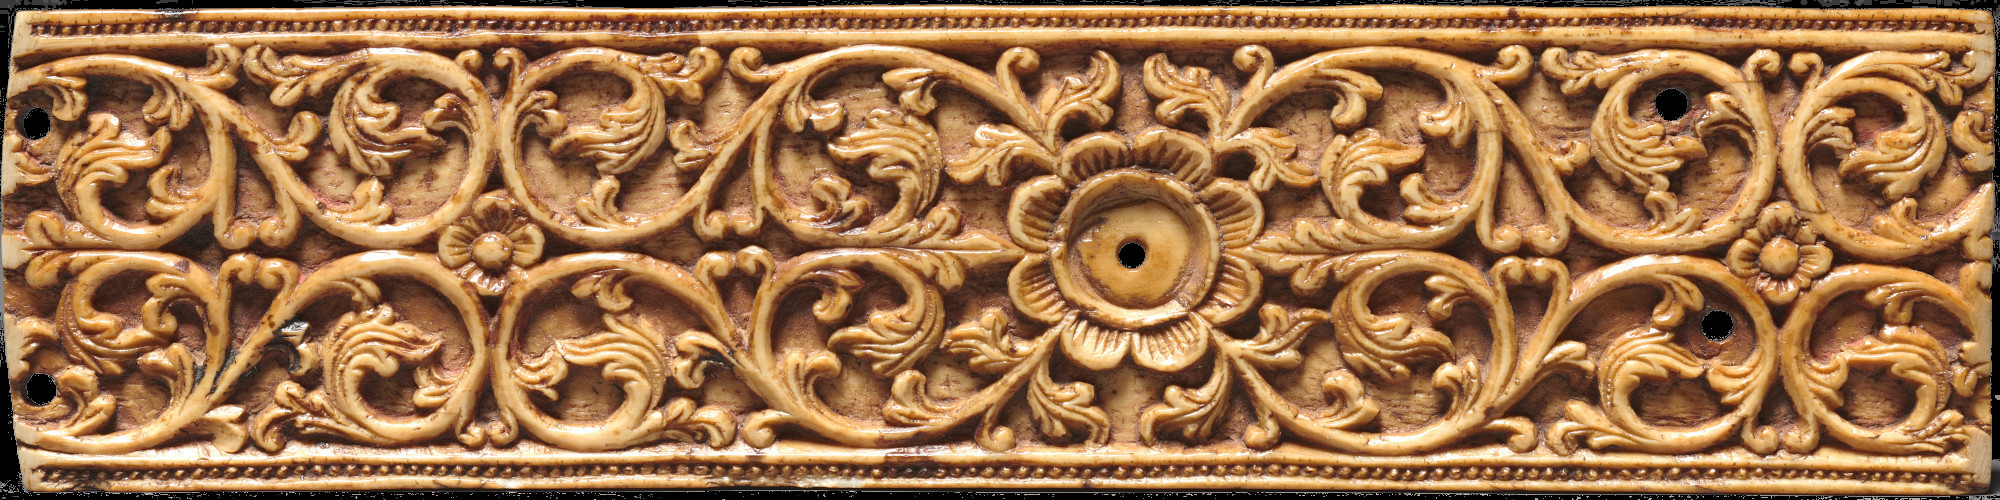
\includegraphics[width=1.2\paperwidth]{ollett-introducing-nesar.jpg}};
      \node[inner sep=0pt] (titlebox) at ([yshift=0.55cm]backgroundimage.north) {\begin{titlebox}\begin{center}\vspace{2ex}%
            \IfFileExists{metadata/metadata-subtitle.tex}{
              {\LARGE\thetitle:\par}\vspace{1ex}
              {\Large\emph{Kolaimaṟuttal} and the Genealogy of Tamil Śaiva Vegetarianism\par}\vspace{2.5ex}
            }{
              {\LARGE\thetitle\par}\vspace{2.5ex}
            }
          {\Large\textit\theauthor\par}\vspace{2ex}
          \end{center}\end{titlebox}};
      \node[inner sep=0pt] (caption) at ([yshift=1cm,xshift=-4.75cm]current page.south east) {\begin{titlebox}[add to width=-6.5cm,fontupper=\linespread{0.75}\selectfont
]%
          {\tiny\raggedright \emph{image source}: Ivory Cover of a Palm-Leaf Manuscript, Sri Lanka, 1600s, Cleveland Museum of Art (via \href{https://commons.wikimedia.org/wiki/File:Ceylon,_17th_century_-_Cover_of_a_Palm-Leaf_Manuscript_-_1992.85_-_Cleveland_Museum_of_Art.tif}{Wikimedia Commons})}%
          \end{titlebox}};

    \end{tikzpicture}
    \vfill
    %{\Large\scshape\press}%
    \end{center}%
    
    \endgroup
  }


\usepackage[linguistics]{forest}
\usepackage{pgfornament}
\usepackage{booktabs,multirow}
\usepackage{wrapfig}
\usepackage{enumitem}
\setlist[itemize]{labelindent=\parindent,itemsep=0.15em,topsep=0pt,leftmargin=\parindent}
\counterwithout{section}{chapter}
\setsecnumdepth{subsubsection}
\maxtocdepth{subsubsection}
\setlength{\cftsectionindent}{1em}
\setlength{\cftsubsectionindent}{1em}
\setlength{\cftsubsubsectionindent}{1em}
\setlength{\parindent}{2em}
\renewcommand{\cftsectionfont}{\bfseries}
\newcommand{\longmark}{{\fontspec{EB Garamond}\raisebox{0.3ex}{ː}\hspace{0.1em}}}
\newcommand{\graph}[1]{{\fontspec{Linux Libertine O}〈#1〉}}
\newcommand{\textgreek}[1]{{\fontspec{GFS Porson}#1}}
\newcommand{\phonet}[1]{{\fontspec{Linux Libertine O}\lbrack#1\rbrack}}
\newcommand{\phonem}[1]{{\fontspec{Linux Libertine O}/#1/}}
\newcommand{\mora}{{\fontspec{GFS Porson}μ}}
\newcommand{\syll}{{\fontspec{GFS Porson}σ}}
\renewcommand{\baselinestretch}{1.1}
\setlength{\RaggedRightParindent}{\parindent}
\frenchspacing
\def\nonfrenchspacing{\frenchspacing}
\AtBeginDocument{\frenchspacing}

\definecolor{formalshade}{rgb}{0.95,0.95,1}
\definecolor{darkblue}{rgb}{0.0, 0.0, 0.55}
\newtcolorbox{pullquote}{
    enhanced,
    boxrule=0pt,
    frame hidden,
    borderline west={2pt}{0pt}{Nesarlinkdark},
    colback=Nesarlinklight,
    sharp corners,
    fontupper=\rmfamily,
    left skip=24pt,
    breakable
    }
\usepackage{xurl}
\usepackage{hyperref}
\hypersetup{pdftitle=\thetitle,
        colorlinks,
        urlcolor=Nesarlink,
        linkcolor=Nesarlink,
        breaklinks=true} 
\usepackage{xurl}
\DeclareRobustCommand{\thinskip}{\hskip 0.16667em\relax}
\def\emdash{—}
\def\d@sh#1#2{\unskip#1\thinskip#2\thinskip\ignorespaces}
\def\Dash{\d@sh\nobreak\emdash}
\def\Ldash{\d@sh\empty{\hbox{\emdash}\nobreak}}
\def\Rdash{\d@sh\nobreak\emdash}

\newcounter{excounter}
\usepackage{hyphenation/nesarhyphenation}
\setcounter{excounter}{1}
\newenvironment{exe}[1]{
\begin{changemargin}{2em}{0em}\noindent\textbf{\theexcounter.\ \ #1}
\end{changemargin}
\begin{changemargin}{4em}{0em}\vspace{-1ex}\noindent\ignorespaces}%
{\end{changemargin}\addtocounter{excounter}{1}}
\widowpenalty10000
\clubpenalty10000

%\usepackage[en]{metre}
%\usepackage{gb4e}
\frenchspacing

\setcounter{page}{1}
\begin{document}
%\RaggedRight

\thispagestyle{empty}
\titleM
\clearpage

\thispagestyle{empty}
\begingroup
\small

\noindent\begin{minipage}[t]{0.8\textwidth}
\noindent\textbf{NEW EXPLORATIONS IN SOUTH ASIA RESEARCH (NESAR)}\smallskip

\noindent An open-access journal of South Asian Studies, founded in 2022.\medskip

\noindent ISSN 2834-3875 \hspace{0.25em} 
\includegraphics[width=0.45cm,align=c]{logoNesar.png} \hspace{0.25em} \url{https://nesarjournal.org}\medskip

\noindent This PDF was generated \today.
\end{minipage}
\begin{minipage}[t]{0.2\textwidth}

\includegraphics[align=t,width=0.5cm]{openaccess.png}
\end{minipage}

\bigskip\bigskip

\noindent\emph{Editorial board}:\smallskip

\noindent\begin{itemize}[itemsep=2pt,parsep=0pt,leftmargin=0.45cm,label={}]
\item Andrew \textsc{OLLETT}, University of Chicago
\item Shubha \textsc{SHANTHAMURTHY}
\item Naresh \textsc{KEERTHI}, Ashoka University
\end{itemize}\medskip

\noindent\emph{Advisory board}:\smallskip

\noindent\begin{itemize}[itemsep=2pt,parsep=0pt,leftmargin=0.45cm,label={}]
\item Diwakar \textsc{ACHARYA}, University of Oxford
\item Richard \textsc{EATON}, University of Arizona
\item Leslie \textsc{ORR}, Concordia University
\item David \textsc{SHULMAN}, Hebrew University of Jerusalem
\item Eva \textsc{WILDEN}, University of Hamburg
\end{itemize}\medskip

\noindent\emph{Principal contact}:\smallskip

\noindent\hspace{0.45cm}Andrew \textsc{OLLETT} (\href{mailto:ollett@uchicago.edu}{\texttt{\color{Nesarlink}ollett@uchicago.edu}})\bigskip\bigskip

\noindent\begin{minipage}[t]{0.48\textwidth}
\begingroup
\tiny\raggedright\noindent
This article is available under a \href{https://creativecommons.org/licenses/by/4.0/}{CC BY 4.0} license. You are free to: 
\begin{itemize}[leftmargin=0.35cm,parsep=0pt,itemsep=0pt]
\item \textbf{Share}: copy and redistribute the material in any medium or format
\item \textbf{Adapt}: remix, transform, and build upon the material for any purpose, even commercially.
\end{itemize}
\noindent under the following terms:
\begin{itemize}[leftmargin=0.35cm,parsep=0pt,itemsep=0pt]
\item \textbf{Attribution}: You must give appropriate credit, provide a link to the license, and indicate if changes were made. You may do so in any reasonable manner, but not in any way that suggests the licensor endorses you or your use.
\item \textbf{No additional restrictions}: You may not apply legal terms or technological measures that legally restrict others from doing anything the license permits.
\end{itemize}\smallskip

\begin{center}

\includegraphics[align=t,width=2cm]{byNesar.png}
\end{center}\smallskip

\tiny\noindent The copyright of this article, as well as all moral rights, rest with the author (\theauthor{}).\vfill

\endgroup
\bigskip
\end{minipage}\hfill
\begin{minipage}[t]{0.48\textwidth}
\begingroup
\tiny
\noindent This PDF file was generated automatically from a source in \href{https://tei-c.org/}{TEI} encoding. The stylesheets used for the transformation are available on \href{https://github.com/nesar-journal/nesar-stylesheets}{this GitHub website}.\medskip

\noindent NESAR uses the \href{https://bombay.indology.info/software/fonts/induni/index.html}{IndUni fonts} designed by John Smith.\medskip

\begin{center}

\includegraphics[width=0.75\textwidth,align=t]{cosas.png}\medskip


\includegraphics[width=0.75\textwidth,align=t]{library.png}
\end{center}\medskip

\noindent NESAR gratefully acknowledges the support of the \href{https://www.lib.uchicago.edu/}{University of Chicago Libraries} and the \href{https://southernasia.uchicago.edu/}{Committee on Southern Asian Studies at the University of Chicago}.\vfill

\endgroup
\end{minipage}
\endgroup
\setcounter{page}{0}
\clearpage

\thispagestyle{firstpage}
\begin{center}
\IfFileExists{metadata/metadata-subtitle.tex}{%
          {\LARGE\thetitle:\par}\vspace{1ex}%
          {\Large\emph{Kolaimaṟuttal} and the Genealogy of Tamil Śaiva Vegetarianism\par}\vspace{1.5ex}%
}{%
          {\LARGE\thetitle\par}\vspace{1.5ex}%
}\bigskip

\begin{tabular}{c}
Andrew Ollett\\[2ex]
{\small\emph{University of Chicago}}\\[1ex]
{\small\href{mailto:ollett@uchicago.edu}{\texttt{ollett@uchicago.edu}}}
\end{tabular}
\end{center}\bigskip

\setlength{\absparsep}{0.5\parskip}
\begin{abstract}
\noindentIn this article, I explore the processes through which Tamil-based Śaivism came to be conceptually equated with the maintenance of a vegetarian diet, a development reflected in the modern Tamil word \emph{caivam} (Skt. \emph{śaiva}), which in colloquial speech primarily signifies lacto-vegetarian cuisine. I contend that although Tamil Śaiva literary sources have long articulated the normativity of vegetarianism, the conflation of Śaiva praxis with plant-based dietary habits likely dates to the late sixteenth and seventeenth centuries. Such, at least, is the picture that emerges from a consideration of the \emph{Kolaimaṟuttal} (\emph{Rejecting Killing}), a brief polemic against animal slaughter likely composed in the then-frontier region of what is now the suburbs of Coimbatore, which emphasizes dietary nonviolence as the quintessential Śaiva virtue and the principal basis for demarcating Śaivism from other religions. A close reading of this hitherto unstudied text suggests that early modern Tamil Śaiva food discourse transformed, at least in part, in response to the emergence of new notions of “self” and “other” in this period, which prompted a corresponding need to rethink the contour and configuration of community boundaries.\medskip

\noindent\textbf{Keywords:} vīraśaiva, madhva, vādirāja tīrtha, vyāsa, desecration, procession, vēdānta, deccan, vyāsantōḷ
\end{abstract}

\pagestyle{nesar}
\clearpage

\begin{KeepFromToc}
  {\small 
  \tableofcontents 
}
\end{KeepFromToc}\bigskip



\raggedbottom
      
\section{Introduction}
      In 2014, a film about a rooster named Baby became a surprise hit among Tamil-speaking audiences. The film, directed by A.\thinskip{}L. Vijay and starring M. Nassar and Sara Arjun, tells the story of a wealthy Ceṭṭi family who have gathered in their ancestral home in Kāraikkuṭi to make an offering to a local deity. Baby (Tm. Pāppā) is both the intended sacrificial victim whose ritual killing promises to eliminate the family’s troubles and an object of affection for the young Tamiḻcelvi (Arjun), granddaughter of the family’s patriarch (Nassar). Through her endearing devotion to the bird, Tamiḻcelvi manages by the final scene not only to save Baby’s life but also to convince her relatives to stop eating meat altogether. Despite its pro-vegetarian message, which in contemporary Tamil society can, in certain contexts, be perceived as an endorsement of Brahminical elitism, the film was a critical and commercial success: at least one leading filmmaker reportedly gave up meat after watching it, and a Telugu remake came out the following year.\footnote{%
Sudha G. Tilak, “Tamil Film on the Explosive Subject of Vegetarianism is a Surprise Hit,” \emph{Scroll.in}, July 12, 2014, \url{https://scroll.in/article/670125/tamil-film-on-the-explosive-subject-of-vegetarianism-is-surprise-hit}.
}



No less striking, at least from the perspective of the history of religions, is the film’s title, \emph{{Caivam}}, which derives from a calque on the Sanskrit \emph{śaiva}, literally, “relating to the deity Śiva.” In colloquial Tamil, however, this term does not first and foremost signify any explicitly religious belief, sentiment, social practice, or institution; its primary referent is lacto-vegetarian food. Countless restaurant signboards across Tamil Nadu, for instance, advertise their establishments’ expertise in preparing \emph{caiva} (“vegetarian”) or \emph{acaiva} (“non-vegetarian”) cuisine. Hence an adequate translation of the film’s title is simply \emph{Vegetarianism}. The film’s moral is consistent with this secularized sense of \emph{caivam}, as the family abandons their entrenched dietary habits not as a result of having received religious teachings, but rather because of the sheer magnetism of Tamiḻcelvi’s childlike ability to love without drawing distinctions between species.


Yet when and how did Tamil Śaiva religion come to be identified with vegetarianism in this manner? Put differently, when and how did the consumption of non-human animals come to be perceived as anathema to established Tamil Śaiva values? And what is the connection between such an understanding and the predominantly nonreligious meaning conveyed by the word \emph{caivam} today?


Indologists have long realized that vegetarianism in India has a history (e.g., \hyperref[Alsdorf2010]{Alsdorf 2010 [1962]}). At least partly in response to the recent political weaponization of diet by Hindu nationalists and related instances of anti-Muslim violence (\hyperref[GhassemFachandi2012]{Ghassem-Fachandi 2012}), both textual scholars and anthropologists have stressed the context-sensitivity and historical contingency of South Asian vegetarian discourse, from ancient Brahminical hand-wringing over Vedic animal sacrifice to modern controversies surrounding cow slaughter (e.g., \hyperref[Bryant2006]{Bryant 2006}; \hyperref[Doniger2009]{Doniger 2009}; \hyperref[Staples2020]{Staples 2020}). It is now widely supposed that the identification of “Hindu” dietary practice with the avoidance of meat is in no small measure a product of the gendered ideologies of the colonial encounter, according to which vegetarian Hindus were often stereotyped as weak and effeminate (\hyperref[Nandy1983]{Nandy 1983}). As one scholar has aptly put it, “[t]hough it is commonplace to regard Hindus as vegetarian and India as the land of vegetarianism from time immemorial, historical scholarship and social fact call these axioms into question; the very meaning of vegetarianism has been, and continues to be, a matter of contestation and of historical and regional variation” (\hyperref[Roy2015]{Roy 2015}: 272).


Nevertheless, much remains unknown about what vegetarianism actually meant to specific religious communities that flourished on the subcontinent during the roughly two-millennia interval between Manu and Gandhi.\footnote{%
For a recent and fascinating discussion of vegetarianism among eighteenth-century Marwari merchants, see \hyperref[Cherian2023]{Cherian 2023}.
}
 This is especially so for Śaiva traditions, which are less commonly associated with dietary nonviolence than their Vaiṣṇava cousins. In order to adequately resist hegemonic and exclusivist representations of Indian food culture as vegetarian, it is essential to address the historical, regional, and sectarian specificity of South Asian attitudes toward the eating of animal flesh.\footnote{%
This idea draws inspiration from \hyperref[Olivelle]{Olivelle}’s (\hyperref[Olivelle1995]{1995}: 374) review of R.\thinskip{}S. Khare’s pathbreaking studies of Indian food culture: “The problem I raise is rather simple: is there a single food ideology which can be termed ‘Hindu’ and which remains constant across time, regions, and sects…? The answer is clearly no.”
}
 The present article endeavors to contribute toward this goal by developing a historically nuanced perspective on representations of vegetarianism in Tamil Śaiva literature through a hermeneutically responsible interrogation of available textual materials.\footnote{%
It must be said here that it is emphatically \emph{not} this paper’s intention to imply that Tamil-speaking Śaivas may have been nonvegetarian before a certain point in time. What people actually ate, or eat, is of comparatively little concern to the arguments elaborated here. 
}



In what follows, I argue that while Tamil Śaiva literature has long articulated the normativity of vegetarianism, it would have been, if not impossible, at least relatively rare to find the fact of being a Śaiva conceptually equated with the maintenance of an exclusively plant-based diet prior to the second half of the sixteenth century. In fact, the earliest explicit attempt to differentiate between Śaiva and non-Śaiva diets in the manner of the modern Tamil antonyms \emph{caivam}/\emph{acaivam} likely dates to roughly a century later. I further suggest that at least one factor that contributed to the drawing of this distinction was the emergence of new notions of “self” and “other” in this period and a corresponding need to rethink the contour and configuration of community boundaries. Facing new social contexts marked by considerable status mobility and intense religious competition, seventeenth-century Tamil Śaiva intellectuals consciously adapted existing forms of vegetarian rhetoric in ways that anticipated discourse about food in modern Tamil. 


An important piece of evidence for this transformation is a brief polemic against animal slaughter entitled \emph{{Kolaimaṟuttal}} (hereafter, \emph{Rejecting Killing}). Probably composed during the late seventeenth century in the vicinity of present-day Coimbatore, in the traditional Tamil region known as Koṅkunāṭu, the text appears to be, with perhaps a single exception, the first independent composition in the Tamil language dedicated to promoting vegetarianism. While admittedly not widely known today, there are reasons to believe that the text played a significant role in making vegetarianism a central feature of Tamil Śaiva identity. It received a lengthy commentary, probably during its author’s lifetime, and thereafter seems to have circulated widely, particularly in the Koṅkunāṭu region.\footnote{%
The text is explicitly mentioned, for instance, in the \emph{{Tiṭṭamalaiyāṇṭavarkommi}}, an eighteenth-century folk ballad (\emph{kummi}) dedicated to Murukaṉ that would have been sung by dancing women at Tiṭṭamalai, a hill about seventy-five kilometers northeast of Coimbatore (\hyperref[Nanacinkaram1986]{Ñāṉaciṅkāram 1986}: 90, v. 97). I would like to thank Cu. Vikṉēcu, a Ph.D. student at Thavathiru Santhalinga Adigalar Arts, Science and Tamil College, for bringing this reference to my attention.
}
 The influential colonial-era Śaiva reformer Āṟumuka Nāvalar (1822–1879) published the text in 1860 (\hyperref[Hudson1992]{Hudson 1992}: 42), and it is likely that the text also served as a key inspiration for the Śaiva mystical poet Irāmaliṅka Aṭikaḷ’s (1823–1874) concept of “compassion for living beings” (\emph{cīvakāruṇyam}).\footnote{%
See \hyperref[Raman2022]{Raman 2022}: 84 and the ensuing discussion.
}



A consideration of the manner in which \emph{Rejecting Killing} creatively responds to a series of established and more recent religious rivals reveals it to be an innovative attempt to navigate conditions then prevalent in the Tamil-speaking dry-zone interior. In particular, it will be demonstrated that the text articulates a novel alimentary ideology, referred to in this article as “Caiva \emph{ahiṁsā},” according to which nonviolence, conceived primarily in terms of vegetarian dietary practices, is represented as the quintessential Śaiva virtue and the principal basis for demarcating the path of Śiva from other, inferior ways of being in the world.\footnote{%
This expression intentionally combines Tamil and Sanskrit transliteration schemes to underscore the text’s indebtedness to both literary traditions. I thank Srilata Raman for first suggesting the phrase to me during a conversation whose date I no longer recall. 
}
 The next section contextualizes the discussion by surveying Tamil Śaiva perspectives on meat eating prior to the seventeenth century. Then follows a section on \emph{Rejecting Killing}’s form and content and another on its engagement with Christian, Śākta, and lay interlocutors. The conclusion offers some brief remarks on the wider significance of food for the early modern consolidation of South Indian Śaivism. 

\section{Situating Caiva \emph{ahiṁsā}}
      In her study of medieval South Indian Buddhist, Śaiva, and Jaina “dietary polemics,” \hyperref[Ulrich2007]{Ulrich} (\hyperref[Ulrich2007]{2007}: 245) has shown that the \emph{{Tēvāram}} poets (circa 6th–8th century) tend to concentrate on the manner in which religious others eat, rather than the kinds of food eaten per se. She convincingly proposes that the rare instances in which the poet Campantar rebukes his adversaries for craving meat target not the well-known nonvegetarianism of Buddhist monastics but rather the sanctimony of Jain ascetics:

\begin{pullquote}
At issue, I suspect, was the perceived hypocrisy of renouncers renowned for an austere vegetarian diet who (allegedly) longed for meat. Most Buddhist monks, in other words, did not insist on vegetarianism, and thus their consumption of meat was perfectly acceptable. Jains, on the other hand, did prohibit meat eating, and therefore desire for it on the part of renouncers might have been viewed as symptomatic of an insufficiency of renunciation.


\medskip\hfill\begin{minipage}{0.9\textwidth}\small\hfill
\hyperref[Ulrich2007]{Ulrich 2007}: 248\end{minipage}\hspace{2em}
\end{pullquote}

Accounting for Campantar’s relative silence on the subject, \hyperref[Ulrich2007]{Ulrich} (249) points to the poet’s “support for Vedic sacrifice” and “valorization of meat eating in a devotional context.” The latter refers to celebrated instances in the lives of certain Tamil Śaiva saints, such as the hunter Kaṇṇappar, whose hagiography is elaborated in the twelfth-century \emph{{Periyapurāṇam}}. While Kaṇṇappar’s life story assumes the transgressiveness of meat (the saint famously offered Śiva a freshly slaughtered boar, to the horror of a Brahmin onlooker), it subordinates dietary norms to devotional intensity (\hyperref[Ulrich2007]{\emph{ibid}.}; \hyperref[Cox2005]{Cox 2005}: 235–236) and the power of austerities performed in previous lives (\hyperref[Monius2004]{Monius 2004}: 156). One might, therefore, summarize the position of the early tradition by saying, as \hyperref[Ulrich2007]{Ulrich} (\hyperref[Ulrich2007]{2007}: 250) does of Campantar, that “absolute nonviolence and vegetarianism were secondary to other values,” of which devotion to Śiva was paramount.


A less flexible position is found in the \emph{{Tirumantiram}}, an assemblage of teachings from the Śaiva Āgamas unlikely to predate the thirteenth century.\footnote{%
On the problems involved in dating this text too early see \hyperref[Goodall1998]{Goodall 1998}:  xxxvii–xxxix.
}
 This text’s initial volume, which celebrates Śiva’s divine instruction and outlines qualifications for entering the path to liberation (\hyperref[Martin1983]{Martin 1983}: 120), contains two adjacent pairs of quatrains under the headings “Not killing” (\emph{kollāmai}, vv. 197–198) and “Rejecting meat” (\emph{pulāṉmaṟuttal}, vv. 199–200).\footnote{%
\hyperref[Natarajan1991]{Natarajan 1991}: 30–31. 
}
 It should be noted that these same topical headings also occur as the titles for two decads in the much earlier \emph{{Tirukkuṟaḷ}} (circa 500 CE), a renowned collection of 1,330 aphorisms on the moral life. These very decads have, in fact, been cited as evidence for the \emph{{Tirukkuṟaḷ}}’s likely Jaina authorship (\hyperref[Zvelebil1973]{Zvelebil 1973}: 157), though every Tamil-speaking religious community has claimed the \emph{{Tirukkuṟaḷ}} as its own. Whatever relationship, if any, the \emph{{Tirumantiram}}’s first volume may bear to the \emph{{Tirukkuṟaḷ}}, it is important to recognize that the former interprets abstention from violence and meat within a decidedly Śaiva theological framework.\footnote{%
The suggestion that Tamil Śaivas adopted vegetarianism from the Jains, or even that they are themselves converted Jains, is a frequently encountered trope in modern Tamil literary histories (\hyperref[Emmrich2011]{Emmrich 2011}: 629).
}
 Thus, v. 197 associates the practice of nonkilling with the worship of one’s guru, and v. 200 suggests that those who have attained Śiva’s feet do not kill or commit other sins. Sandwiched between these are two conceptually similar stanzas, the second of which is possibly the earliest explicit condemnation of nonvegetarianism in Tamil Śaiva literature:

\begin{pullquote}\raggedright
      \emph{pollāp pulālai nukarum pulaiyarai}\\
\emph{ellāruṅ kāṇa iyamaṉ ṟaṉ tūtuvar}\\
\emph{cell ākap paṟṟit tī vāy narakattil}\\
\emph{mallākkat taḷḷi maṟittu vaippārē}
\end{pullquote}
      
\begin{pullquote}


	
	    For all to see, Yama’s messengers quickly\\
	    seize the outcastes who consume foul flesh,\\
	    push them on their backs in the fiery maw of hell,\\
	    and keep them there.\footnotemark{}
	  

\medskip\hfill\begin{minipage}{0.9\textwidth}\small\hfill
\emph{{Tirumantiram}} v. 199\end{minipage}\hspace{2em}
\end{pullquote}\footnotetext{All translations, unless otherwise noted, are mine. \emph{cellāka}, translated here as “swiftly,” could also be translated “as they die” (“who consume foul flesh as they die”).
}

Later Śaiva authors repeatedly returned to the themes iterated in this quatrain, which links meat eaters with lowly birth and vividly depicts the terrible fate awaiting them after death. In context, v. 199 can be interpreted to suggest that maintaining a vegetarian diet is necessary in order to be eligible for receiving Śiva’s liberating grace and avoiding an unpleasant rebirth. While this is clearly distinct from the stance adopted in the \emph{{Tēvāram}}, dietary nonviolence is hardly portrayed as the archetypal Śaiva virtue in the \emph{{Tirumantiram}}. Rather, it is accorded roughly the same importance as a host of other good qualities mentioned in the first volume, including equanimity, devotion, generosity, sexual continence, and abstention from alcohol.


Expressions of the evils of eating meat become noticeably more common during the late sixteenth century. Two Tamil texts from this period are particularly rich sources for such statements. The first is the \emph{{Kācikaṇṭam}}, an adaptation of the \emph{{Kāśīkhaṇḍa}} on Benares, which became widely distributed in South India shortly after its circa mid-fourteenth-century composition (\hyperref[Minkowski2002]{Minkowski 2002}: 331–332). The second is the \emph{{Civatarumōttaram}}, an influential translation of the circa sixth–seventh-century \emph{{Śivadharmottara}} on lay Śaiva praxis.\footnote{%
\hyperref[Ganesan2009]{Ganesan 2009}: 36–38 summarizes the Tamil text, the \emph{opus magnum} of Citamparam-based scholar Nigamajñāna I. 
}
 Both texts denounce killing and consuming animals in the context of delineating forms of behavior (in)appropriate for uninitiated Śaiva householders. While the precise relationship between these works and their respective Sanskrit source materials awaits further study, for now it can be said that the \emph{{Kācikaṇṭam}} and \emph{Civatarumōttaram} supported, as proof texts, the development of a ritual-prescriptive framework for theorizing and policing the dietary practices of lay Śaivas in South India.\footnote{%
A research project underway at L’Orientale University of Naples is studying the transmission and reception of the vast \emph{Śivadharma} corpus across premodern South Asia and promises to transform our understanding of the \emph{Civatarumōttaram} and its Sanskrit prototype. In September 2022, I had the opportunity to read portions of \emph{Rejecting Killing }and its commentary with members of this group, for which I wish to thank Florinda De Simini and Margherita Trento. I have since begun examining the \emph{{Civatarumōttaram}}’s negative appraisal of nonvegetarianism, which appears to depart significantly from the position of the \emph{Śivadharmottara}. These findings will be published along with a translation of the \emph{{Civatarumōttaram}}’s sixth chapter that I am currently preparing.
}



An intriguing treatment of vegetarianism from this period is also found in the \emph{{Civañāṉatīpam}} (\emph{Lamp on Śiva-Gnosis}), a philosophical text incorporating elements of Śaiva Siddhānta, Advaita Vedānta and Vīraśaivism.\footnote{%
\hyperref[Arunacalam2005]{Aruṇācalam 2005 [1975]}: 269–275 provides information on this text. He is skeptical of the claim that the text’s reputed author, Rēvaṇa Cittar, was a Vīraśaiva Brahmin, suggesting he followed the Śaiva Siddhānta (95–98), though by his own admission (271) the \emph{{Civañāṉatīpam}} includes references to distinctively Vīraśaiva practices such as \emph{liṅgadhāraṇa}. The verse translated below seems to support a claim for the work’s Vīraśaiva provenance, though a thorough textual study remains a desideratum. 
}
 After discussing how Śiva dispenses his grace to different types of enfettered souls, the text’s “General” (\emph{potu}) section praises the abandonment of killing and other vices before addressing the issue of food: 

\begin{pullquote}\raggedright
      \emph{evvuyirum parāparaṉ cannitiyat’ ākum}\\
\emph{ilaṅkum uyir uṭal aṉaittum īcaṉ kōyil}\\
\emph{evvuyirum emmuyir pōl eṉṟu nōkkiy}\\
\emph{iraṅkātu koṉṟ’ aruntum iḻiviṉōrai}\\
\emph{vavvi yamaṉ tūtar arun taṇṭañ ceytu}\\
\emph{vall irumpaiy urukkiy avar vāyil vārttu}\\
\emph{vevviya tīy eḻu narakil vīḻtti māṟā}\\
\emph{vētaṉai ceyt’ iṭuvar eṉav ōtu nūlē}
\end{pullquote}
      
\begin{pullquote}


	
	    Every living being is the sacred presence of the Supreme.\\
	    All bodies of manifest living beings are the temple of the Lord.\\
	    As for the base ones who kill and eat,\\
	    not thinking with compassion upon living beings as they do their own lives,\\
	    The messengers of Yama will take hold of and punish them severely,\\
	    melting hard iron and pouring it in their mouths,\\
	    making them fall into the seven hells of searing fire\\
	    and causing them ceaseless pain.\\
	    Thus declares the treatise. 
	  

\medskip\hfill\begin{minipage}{0.9\textwidth}\small\hfill
\emph{Civañāṉatīpam} v. 11 (\hyperref[Atikalaciriyar1970]{Aṭikaḷāciriyar 1970}: 10)\end{minipage}\hspace{2em}
\end{pullquote}

Lines 3–8 adapt the fire and brimstone message of \emph{{Tirumantiram}} v. 199 (presumably the cited “treatise”), dilating graphically upon the tortures awaiting nonvegetarians in hell. The initial two lines, however, are reminiscent of the Kannada Vīraśaiva \emph{vacana} corpus  \Dash  notionally dating to the twelfth century but in any case available to intellectuals in the sixteenth (see \hyperref[ChandraShobhi2005]{Chandra Shobhi 2005} and Ben-Herut this issue)  \Dash  a central theme of which is the notion that the body constitutes the true Śiva temple.\footnote{%
\hyperref[Ramanujan1973]{Ramanujan 1973}: 19–22. For a recent critical assessment of Ramanujan’s reading of the \emph{vacana}s see \hyperref[BebHerut2018]{Ben-Herut 2018}: 5–10.
}
 Striking for their uncompromising universalism, these two lines have entered the proverbial repertoire of learned Tamil speakers, though their origins are largely forgotten (\hyperref[Arunacalam2005]{Aruṇācalam 2005 [1975]}: 273–274). Taken as a whole, this verse expands the theological significance of vegetarianism by associating the condemnation of meat eaters with a reflection on the very nature of living beings and their embodied forms. If all bodies are Śiva temples, then to be vegetarian is to actively care for the deity’s sacred abode and the divine presence that dwells within it, while to be otherwise is to desecrate the same. Moreover, by foregrounding this idea at the beginning of its exposition of Śiva-gnosis, the text implies that vegetarianism is not simply one of the virtues a Śaiva must cultivate but rather the very sine qua non of liberation.


If this admittedly brief survey demonstrates anything, it is that vegetarianism became a more conspicuous and theologically weighty topic in Tamil Śaiva sources in the century immediately preceding the composition of \emph{Rejecting Killing}. It is to the latter’s explicit theorization of the difference between Śaiva and non-Śaiva diets in terms of the renunciation of meat to which this article now turns.

\section{The Vegetarian’s Apotheosis}
      \emph{Rejecting Killing }is a tour de force of concision, consisting of just twenty-two stanzas composed, with the exception of an initial benedictory verse (not counted toward the total), in \emph{āciriya viruttam} meter. Tradition identifies its author, unmentioned in the text itself, as Cāntaliṅka Cuvāmikaḷ, a Vīraśaiva intellectual active in the latter half of the seventeenth century (\hyperref[Steinschneider2016]{Steinschneider 2016}: 301; \hyperref[UranAtikal2009]{Ūraṉ Aṭikaḷ 2009}: 55–64). Cāntaliṅka is credited with establishing a monastic institution at Pērūr, a temple town located on the western edge of present-day Coimbatore, and text-internal evidence supports the hypothesis that \emph{Rejecting Killing} is a product of the early modern Tamil hinterlands.\footnote{%
The allusion in v. 6 to Jesuit criticisms of the doctrine of rebirth and a Śaiva response to the same suggests that the text could not have been composed prior to the mid-seventeenth century. The \emph{terminus ante quem} is less certain. However, in the absence of contradicting evidence, it seems reasonable to accept the traditionally posited late-seventeenth-century date. Taken together, the text’s allusion to Christianity, preoccupation with Śākta blood sacrifice, and agrarian slant strongly suggest an early modern dry-zone context, and accord quite well with what is known of Koṅkunāṭu society at that time. For a detailed anthropological study of this region see \hyperref[Beck1972]{Beck 1972}. 
}
 The text received a single, lengthy commentary, also anonymous, which is traditionally attributed to Cāntaliṅka’s grand-disciple, Citampara Cuvāmikaḷ of Tiruppōrūr.


The text’s title, given in a densely packed first verse along with virtually all the information traditionally provided at the beginning of a Tamil scholastic treatise, hints at the work’s hybrid form while still managing to appear entirely conventional. \emph{{Kolaimaṟuttal}} is a kind of portmanteau of “Not killing” (\emph{kollāmai}) and “Rejecting meat” (\emph{pulāṉmaṟuttal}), recalling, of course, the aforementioned passages of the \emph{{Tirumantiram}} and \emph{{Tirukkuṟaḷ}}. However, the verb \emph{maṟuttal}, according to the University of Madras \emph{Tamil Lexicon} (s.v.), can also mean “to confute, refute the opinion or argument of another,” suggesting the text’s concern to counter other religious traditions’ justifications for animal slaughter. This innovative blending of dietary didacticism with formal religious polemics in the guise of a profound traditionalism is crucial to the text’s social agenda, to be examined in further detail below.\footnote{%
It should be noted that, as an independent text dedicated to denouncing nonvegetarianism, \emph{Rejecting Killing} has virtually no precedent in Tamil literary history. The commentary occasionally cites from another text entitled \emph{{Pulāṉmaṟuttal}} (\emph{Rejecting Meat}, not to be confused with the identically named chapter of the \emph{{Tirukkuṟaḷ}}), about which I have unfortunately failed to uncover any relevant information.
}



Another important feature of the text is its narrative frame, introduced in the second verse, around which the discourse is carefully organized. Enhancing the coherence of this frame is the employment, also initiated in v. 2, of a form of versification called \emph{antāti}, in which the last word of each stanza supplies the first word for the following one:

\begin{pullquote}\raggedright
      \emph{eṭutt’ uḷav eccamayikaḷum ulakaruñ cār ōr avaiyiṉ iṭaiyiṟ ṟōṉṟum}\\
\emph{uṭut taṉaic cūḻ tara viḷaṅku matiyiṉ uyar caivarai vant’ oruvaṉ ṟāḻnt’ īṇṭ’}\\

\clearpage
\emph{aṭutta palav uyirt tōṟṟatt’ uyarvu tāḻv’ aruḷuk’ eṉav avaṉait tēṟṟit}\\
\emph{taṭutta puṟac camayikaṭk’ uttaram uṟutti niṟuttukiṉṟār tampāl ūṟṟam}
\end{pullquote}
      
\begin{pullquote}
A man approached an eminent Śaiva who, like the moon shining in the midst of stars, appeared in the center of an assembly where gathered adherents of all the established religions as well as common folk.\medskip


Bowing, he said, “Please explain the relative status of the many forms living beings assume in this world.”\medskip


Clarifying the matter for him, [the Śaiva] furnished replies to the adherents of the heteroprax religions who opposed him and established the certitude of his position.\footnotemark{}


\medskip\hfill\begin{minipage}{0.9\textwidth}\small\hfill
\emph{Rejecting Killing} v. 2 (\hyperref[CantalinkaCuvamikal1927]{Cāntaliṅka Cuvāmikaḷ 1927}: 3)\end{minipage}\hspace{2em}
\end{pullquote}\footnotetext{I have translated this verse in the past tense, though it uses the grammatical present.
}

Among those assembled at this seventeenth-century South Indian World’s Parliament of Religions are representatives from the “outer religions” or \emph{puṟa-c camayaṅkaḷ}. This is a technical term used in Tamil Śaiva Siddhānta polemics to differentiate between traditions that do not acknowledge the authoritativeness of Vedic and Śaiva Āgamic revelation and the “inner religions” (\emph{aka-c camayaṅkaḷ}) that do. The \emph{locus classicus} for this distinction is the circa thirteenth-century philosophical treatise \emph{{Civañāṉacittiyār}}, a text that is partially structured as a systematic refutation of fourteen rival schools (\emph{parapakkam}), and partially as an elaboration of the established doctrine (\emph{cupakkam}). Of note here is the way in which \emph{Rejecting Killing} subtly begins to refocus the meaning of heteropraxy around a rejection of what is perceived to be the settled position of divine revelation on matters of dietary practice. Following, for the most part, the twofold pattern established in the \emph{{Civañāṉacittiyār}}, the Śaiva will illuminate the nature of alimentary orthopraxy by rebutting the claims of his opponents and expounding the conclusion accepted by the tradition.\footnote{%
\emph{Rejecting Killing}’s polemical form is likely inspired by a brief reference to Buddhist nonvegetarianism in the \emph{{Civañāṉacittiyār}}. In the latter’s rebuttal of Sautrāntika Buddhism, the text makes the opponent claim that while killing is unacceptable (it had been celebrated by the previous opponent, the Materialist, at \emph{parapakkam} v. 36, \hyperref[Balasubramanian2013]{Balasubramanian 2013}: 130–131), eating creatures killed by another is not, since what is dead is insentient and since the demerit of killing accrues only to the killer, not the eater (v. 92, 178). The text responds, from the perspective of the accepted position, by placing responsibility for the sin that accrues to the butcher squarely on the Buddhist, since it is for the latter’s sake that animals are killed. The opponent is then portrayed as a hypocrite thrice over: accumulating sins for one who feeds him, he lacks austerity; he eats meat but does not offer the same to his deity; and he is disgusted by his own bodily impurity but not that of the creatures he eats (v. 131, 220–221). As in Campantar’s dietary polemics, it is not meat-eating per se, but rather the Buddhist’s purported deficiency of austerity, as well as his ritual inconsistency, that is singled out for ridicule. Nonetheless, the explicit reference to another tradition’s support for nonvegetarianism in a formal \emph{pūrvapakṣa}/\emph{siddhānta} context can be understood to have anticipated the approach adopted in \emph{Rejecting Killing}.
}



Also present are common folk (\emph{ulakar}, lit. “worldly people”) whose religious identity is unmarked. Presumably the anonymous man (\emph{oruvaṉ}) in v. 2, who serves as the text-internal witness to the imminent public exchange, also belongs to this group. Indeed, the conceit of the assembly (\emph{avai}, Skt. \emph{sabhā}) appears designed to draw attention to this questioner. One could conceive of a hypothetical scenario in which the text omitted v. 2 and proceeded directly to elaborating and defending its core position; what would be lost is precisely this spectator, whose implied conversion to vegetarianism toward the end of the text constitutes a kind of narrative climax. This suggests that the common folk are closely linked to the text’s intended audience. The latter are identified in v. 1, which proclaims that \emph{Rejecting Killing} was composed “so that those who fear the fire [of hell] will reject killing and attain virtue” (\emph{añciṉar tīkk’ aṟaṅ kolaimai taḷḷi-c cārtaṟk’}). Thus, the text can be said to imagine an audience of nonvegetarians, unaffiliated to any specific religious tradition, who nevertheless are at least potentially receptive to the authority of revealed Śaiva scriptures on the matter of correct dietary discipline. 


Verse 3 gives the Śaiva’s reply to the man’s question and is the pivot of the text:

\begin{pullquote}\raggedright
      \emph{ūṟṟa mikuñ carācarattuḷ uyarcci carañ carattu ṇarar narar tamm uḷḷum}\\
\emph{ēṟṟamun tāḻcciyum uḷa pall uyir cekutt’ uṇṭ’ uṭalai vaḷartt’ iṭuṅ kīḻ ammēl}\\
\emph{cāṟṟum uyirk kolai purita ṟuyar neṭu nāḷ eṉṟum uṭa ṟāṉ poyy eṉṟun}\\
\emph{tēṟṟa mikk’ ēṉṟ’ uyir tamai vīṭṭiṉum avaṟṟiṉ uyir purakkun tīt’ ilōrē}
\end{pullquote}
      
\begin{pullquote}
	    Among immobile and mobile beings\\
            that possess [comparatively] greater intelligence,\\
	    mobile beings are superior.\\
	    Among mobile beings, men.\\
            There is superiority and inferiority among men as well.\\
	    Lowly men (\emph{kīḻ}) nourish their bodies,\\
            killing and eating many living beings.\\
	    Above them are the faultless ones who,\\
            accepting with complete certainty that killing\\
            the aforementioned living beings yields sorrow for a long time,\\
	    and that the body itself is false,\\
	    protect those beings’ lives even if it costs them their own.
	  

\medskip\hfill\begin{minipage}{0.9\textwidth}\small\hfill
\emph{Rejecting Killing} v. 3  (\hyperref[CantalinkaCuvamikal1927]{Cāntaliṅka Cuvāmikaḷ 1927}: 4)\end{minipage}\hspace{2em}
\end{pullquote}

This verse elaborates a chain of being whose structure can be represented in tabular form:


\begin{table}[ht!]\label{tab1}\centering
\caption{The chain of being according to \emph{Rejecting Killing}, v. 3}
\begin{tabular}{l}\toprule

	
	1. Vegetarian humans \\
      
	2. Nonvegetarian humans \\
      
	3. Mobile beings (non-human animals) \\
      
	4. Immobile beings (plants) \\\bottomrule
      
      
\end{tabular}
\end{table}
      

The significance of this classificatory scheme hinges on the fact that it constitutes a response to a question concerning the relative rank of “the many forms living beings assume in this world” (\emph{īṇṭ’ aṭutta pala-v uyir-t tōṟṟatt’}). In its primary sense, the phrase \emph{uyir-t tōṟṟam}, literally “appearance of living beings,” refers to a common taxonomy according to which creatures are grouped on the basis of their mode of generation, namely, egg-born (Skt. \emph{aṇḍaja}), moisture-born (\emph{svedaja}), sprout-born (\emph{udbhijja}), and womb-born (\emph{jarāyuja}). Both this fourfold system (Skt. \emph{bhūtagrāma}) and the twofold division of beings into “immobile” and “mobile” categories are found at the beginning of the ancient Ayurvedic treatise \emph{{Suśrutasaṁhitā}}, though they also appear in other contexts, notably the epics and \emph{dharmaśāstra}, where they are often linked to the process of the Self’s transmigration through different forms of embodied being (\hyperref[Zimmerman1987]{Zimmerman 1987}: 199). The concept was appropriated within specific soteriological traditions, and frequently recurs in contexts emphasizing the rarity of human birth and the need to use one’s time to pursue liberation. For instance, the \emph{{Civañāṉacittiyār}} (\emph{cupakkam}, vv. 179–181) refers to the \emph{uyir-t tōṟṟam} while explicating the process by which Śiva causes the soul to pass through an elaborate series of embodiments across hundreds of thousands of lifetimes, culminating in one’s birth as a man in a middle-class Śaiva family in India. The distinction between vegetarian and nonvegetarian humans also came to be folded into such accounts of the transmigratory process, likely not much prior to \emph{Rejecting Killing}’s composition. Thus, the circa fifteenth-century religious anthology \emph{{Peruntiraṭṭu}} (1912, \emph{arumaiyuraittal}, v. 6, 30), charting the path of the Self to the highest form of embodiment (namely, a Brahmin male in the Cōḻa country who understands the Vedānta), stresses the rare good fortune of not being born among meat eaters in the hill country.


\emph{Rejecting Killing} synthesizes this tradition of reflection on the soteriological significance of the \emph{uyir-t tōṟṟam} with teachings adapted from the \emph{{Tirumantiram}} and especially the \emph{{Tirukkuṟaḷ}}. These include the ideas (1) that meat eaters are low-born or base and selfishly seek to sustain their bodies with those of other beings (\emph{{Tirukkuṟaḷ}} v. 329, v. 251); and (2) that the wise realize that killing leads to unfortunate rebirths and are aware of the impermanence of the body, which is not worthy of nourishing at the cost of others’ lives, and who therefore would rather forfeit their life than take another’s (\emph{{Tirukkuṟaḷ}} v. 255, v. 325, v. 330, v. 338, v. 340, v. 327). Fusing taxonomy with ethical insight, the Śaiva thus presents vegetarians as the pinnacle of embodied existence. 


Crucially, the absence of explicit sectarian content and repeated paraphrasing of the \emph{{Tirukkuṟaḷ}}, which is viewed as authoritative by all Tamil-based religious traditions, suggests the Śaiva has carefully formulated his response to be comprehensible to his relatively untutored audience, that is, the layman of v. 2 who does not yet understand this hierarchy and who is therefore still unsure about how he should live.\footnote{%
The commentary to v. 2 suggests as much, claiming the Śaiva speaks “so that all the people gathered in the assembly, from child to pandit, can agree” (\emph{accapaiyiṉ irunt’ uḷḷa āpālapaṇṭitar ākiya carva caṉaṅkaḷukkuñ cammatam varumpaṭiyē}, p. 4). 
}
 In apparent anticipation, then, of the modern sense of \emph{caivam} in colloquial speech, which as mentioned above has largely been shorn of its earlier religious connotations, v. 3 establishes a nonsectarian theory of vegetarian supremacy that is nevertheless presented as originating from a Śaiva source. This framing of Caiva \emph{ahiṁsā} as a universal value constitutes, I would suggest, a new understanding of vegetarianism in Tamil Śaiva thought, one that views it as pertinent not only to brahmins, monastics, ascetics, or even lay Śaiva householders, but rather, like A.\thinskip{}L. Vijay’s \emph{{Caivam}}, to all people. In the conclusion, I will link this formulation to what I see as the text’s attempt at establishing a meatless public in the frontier region of late seventeenth-century Koṅkunāṭu.


Nevertheless, the bulk of \emph{Rejecting Killing} defends the vegetarian’s superiority on decidedly religious grounds, above all by countering objections raised by representatives of the “outer religions.” A stylistic peculiarity of the text, however, is that the identity of these interlocutors and their counterarguments are not, for the most part, made explicit. More specifically, although the text maintains the situation of oral interreligious debate through periodic usage of the grammatical second person (e.g., “your words are mistaken,” \emph{uṉ coṟ piḻai-y ām}, v. 6), it tends to relate only the established conclusion (\emph{uttarapakṣa}/\emph{siddhānta}), omitting most of the various opponents’ prima facie positions (\emph{pūrvapakṣa}). While the basic gist of the text is often clear enough, an adequate understanding is frequently impossible without the aid of a commentary, which must supply the unstated “questions” to which the Śaiva responds.\footnote{%
The commentary observes its own necessity in its introduction to v. 4, noting that the meaning of the base text is dependent upon a “syntactical expectancy” (\emph{avāynilai}, p. 7).
}



In this sense, \emph{Rejecting Killing }mimics the conventions of scholastic Sanskrit, specifically the ancient \emph{sūtra}/\emph{bhāṣya} model that facilitates the memorization of the main points of a particular system of thought (\hyperref[Tubb2007]{Tubb and Boose 2007}: 2). It thus seems likely that the text was designed to be memorized by a predominantly nonvegetarian audience, such as literate members of a rural peasantry. It is possible that Cāntaliṅka himself would have provided the original, oral exegesis of the text. However, his hagiography suggests that he commissioned the learned scholar Tiruppōrūr Citampara Cuvāmikaḷ, his disciple’s student, to compose commentaries for \emph{Rejecting Killing} and other works, implying that he intended the text to be read in conjunction with Citampara Cuvāmikaḷ’s written commentary. The ensuing discussion inevitably makes use of this gloss to elucidate the text’s polemics. 


Whatever the case may be, the Śaiva defends his position in a highly systematic manner. The commentary clarifies the overall pattern of the arguments by identifying the interlocutors and their prima facie claims. \hyperref[tab2]{Table 2} summarizes the relevant information.

\begin{table}[ht!]\label{tab2}\centering
\caption{Interlocutors and prima facie claims refuted in \emph{Rejecting Killing}, as specified by the commentary}
\renewcommand{\arraystretch}{1.5}
\begin{tabularx}{\textwidth}{>{\hangindent=2em\raggedright\arraybackslash}Xl>{\hangindent=2em\raggedright\arraybackslash}X}\toprule
\textbf{Interlocutor} &\textbf{Passage} &\textbf{Synopsis}\\\midrule
	  
	  1. a Materialist (\emph{ulōkāyataṉ}) &
	  vv. 4–5 &
	  Killing is acceptable.
	 \\
      
	  2. a Christian (\emph{ēcumatavāti}) &
	  v. 6 &
	  Killing non-human animals is acceptable.
	 \\
      
	  3. a “left-handed” tantric practitioner (\emph{vāmi}) &
	  vv. 7–16 &
	  Killing animals in tantric ritual contexts is acceptable.
	 \\
      
	  4. three Buddhists (\emph{pauttar}) &
	  vv. 16–17 &
	  Eating the meat of animals one has not personally killed is acceptable.
	 \\
      
	  5. six common folk (\emph{laukikar}) &
	  vv. 17–19 &
	  Eating meat for reasons of emergency, health, or custom is acceptable.
	 \\
      
	  6. the man from v. 2, who has become spiritually mature (\emph{pakkuviyāṉavaṉ}) &
	  vv. 20–22 &
	  It is acceptable if one’s kin eat meat.
	 \\\bottomrule
      
\end{tabularx}
\end{table}
      

The polemic thus advances in a logical sequence, its target moving (sometimes mid-verse) from the extreme claim that killing is intrinsically permissible to a series of progressively more qualified stances that accept killing in specific contexts, or that reject killing as such but permit the consumption of animal flesh under certain conditions. The text thus reveals the truth gradually, which makes sense given its didactic aims.\footnote{%
This progressive organizational structure is typical of many South Asian doxographical texts, including the final sections of the Tamil \emph{{Maṇimēkalai}} and the Sanskrit \emph{{Sarvadarśanasaṅgraha}}, as \hyperref[Nicholson2010]{Nicholson} (\hyperref[Nicholson2010]{2010}: 150–151) points out, though he would probably categorize \emph{Rejecting Killing} as a form of religious polemic rather than doxography. An alternative way of arranging philosophical difference can be found in the Jain scholar Haribhadrasūri’s “argumentatively neutral” \emph{{Ṣaḍdarśanasamuccaya}}, recently discussed by \hyperref[Mundra2022]{Mundra 2022}.
}
 Conspicuously absent from the list of interlocutors are the Jains. Presumably this is because they are known to reject nonvegetarianism in all circumstances, unlike Tamil Śaivas, who, as noted, traditionally recognize its legitimacy within certain Vedic sacrificial and devotional contexts. The Jains, therefore, would according to the text’s internal logic have to be positioned “higher” in the hierarchy than the Śaiva, which is clearly unacceptable. Of the interlocutors who \emph{are} listed in \hyperref[tab2]{Table 2}, numbers 2, 3, and 5 constitute relatively new quarries for Tamil Śaiva polemicists. The next section analyzes the Śaiva’s arguments against these implied opponents and explores their relevance for the formation of Caiva \emph{ahiṁsā}.

\section{Christians, Sorcerers, and Other Killers}
      In response to an implicit defense of killing, vv. 4–5 claim that causing the death of living beings leads to rebirth in hell and supply arguments for the existence of an immaterial soul capable of experiencing the fruits of action after death.\footnote{%
Cf. the link between Materialism and killing established in the \emph{{Civañāṉacittiyār}} (\emph{parapakkam} v. 36) and the latter’s refutation of the Materialist denial of the soul (\emph{parapakkam} vv. 38–55).
}
 The verse that follows, according to the commentary, answers a Christian’s counter that although murder leads to hell, killing non-human animals is permissible because in the Bible (\emph{cattiya vētattil}, 16) it is said that God made animals for the benefit of mankind. For the sake of clarity, the following translation numbers sentences by subscript (S\textsubscript{1}, S\textsubscript{2}, etc.) and the ensuing exegesis uses conditional clauses to mark information supplied in the commentary.

\begin{pullquote}\raggedright
      \emph{tēc’ iṟai māṉuṭarkk’ evaiyum aruḷiṉ uṇṭ’ īk kīṭam aiy eṉ ceyvāy māntarkk’}\\
\emph{āc’ aruḷvat’ eṉai vēṅkaiy ātiy accātikaḷ avar coṟk’ aṭaṅkum āṟ’ eṉ}\\
\emph{kāc’ aṭaint’ immuṟaiyum ōr ōr kāṟ ṟirivat’ eṉai muṉañ cey karuman taṉṉāṟ}\\
\emph{pēcum acarātiy uruv uyirkaḷ uṟal uṇmaiy uṉ coṟ piḻaiy ām aṉṟē}
\end{pullquote}
      
\begin{pullquote}
\textsubscript{1}If the radiant Lord granted all [animals] to men, what do you do with the worm that is [spawned by] a fly [on excrement, or other] minute [creatures]? \medskip


\textsubscript{2}Why does He trouble men with tigers, etc.?\medskip


\textsubscript{3}How is it that certain species obey men’s command?\medskip


\textsubscript{4}Why does even this system become flawed and inconsistent in particular instances? \medskip


\textsubscript{5}It is true that souls assume the form of the aforementioned immobile beings, etc., according to actions performed in previous [births].\medskip


\textsubscript{6}Your words are mistaken, are they not? (v. 6, p. 17)


\medskip\hfill\begin{minipage}{0.9\textwidth}\small\hfill
\emph{Rejecting Killing} v. 6  (\hyperref[CantalinkaCuvamikal1927]{Cāntaliṅka Cuvāmikaḷ 1927}: 17)\end{minipage}\hspace{2em}
\end{pullquote}

S\textsubscript{1}–S\textsubscript{4}, which rebuts the Christian’s contention, constitutes a highly elliptical paraphrase of three stanzas, cited in the gloss, from an otherwise lost anti-Christian polemic entitled \emph{{Ēcumatanirākaraṇam}} (\emph{Refutation of the Jesus-Doctrine}).\footnote{%
For a translation and discussion of these verses see \hyperref[Trento2022]{Trento 2022}: 291–294.
}
 Tradition attributes this text  \Dash  perhaps the first of its kind in the Tamil language  \Dash  to the seventeenth-century Vīraśaiva poet Tuṟaimaṅkaḷam Civappirakācar, who is remembered to have been Cāntaliṅka’s brother-in-law. While the polemic’s composition has been linked to a supposed meeting between Civappirakācar and the Italian Jesuit Constanzo Gioseffo Beschi (1680–1747), \hyperref[NilakantaSastri1958]{Nilakanta Sastri} (\hyperref[NilakantaSastri1958]{1958}: 379) rejects this possibility, and as discussed below the paraphrased verses are better understood as a reply to ideas found in earlier texts attributed to Roberto de Nobili. 


S\textsubscript{1} is clear: tiny creatures serve no obvious human purpose. If one claims that they supply food for larger animals that do, S\textsubscript{2} asks why some of the latter harm mankind. If it is answered that animals do not submit to human will because God cursed the first man (i.e., Adam) for his disobedience, S\textsubscript{3} replies by pointing out that some species, such as cows, do obey men. If one retorts that God ordained it such that certain species would submit to men’s will while others would not, S\textsubscript{4} responds by alluding to the fact that humans are sometimes obeyed by proverbially dangerous creatures such as snakes and sometimes killed by proverbially submissive animals such as cows. Finally, S\textsubscript{5} (not part of the paraphrase) affirms the established conclusion, namely that human relations with other forms of life are governed not by the curse of a divine creator but rather the doctrine of transmigration.


Arguments against rebirth are a recurring theme in the writings of the Madurai-based Jesuit Roberto de Nobili (1577–1656).\footnote{%
\hyperref[Rajamanickam1972]{Rajamanickam 1972} gives an overview of de Nobili’s life and writings.
}
 Departing from earlier missionary tactics, which prioritized the conversion of low-caste communities, de Nobili (in)famously fashioned himself after the manner of a Brahmin ascetic and wrote Tamil in a style calibrated to engage learned audiences, especially Śaivas.\footnote{%
\hyperref[Clooney1988]{Clooney 1988}: 32. A letter discussed by \hyperref[Zupanov1999]{Županov} (\hyperref[Zupanov1999]{1999}: 153–157) demonstrates that as early as 1607 de Nobili had attempted to disabuse an upper-caste Śaiva Siddhāntin of his faith in rebirth.
}
 Although his criticisms of rebirth are, like those of other contemporary Jesuits, framed in strictly philosophical terms (\hyperref[Clooney2014]{Clooney 2014}), in certain of his writings they occur in the context of discussions that allude to biblical accounts of humanity’s God-given dominion over the animals and the latter’s rebellion that was precipitated by the Fall. This is the case, for instance, in de Nobili’s \emph{{Ñāṉōpatēcam}}, a summation of his great Catechism: 

\begin{pullquote}
This smaller \emph{{Ñāṉōpatēcam}}’s seventh chapter is about the creation of the “first mother” and “first father”  \Dash  Eve and Adam, we might say  \Dash  and their sin and the resultant original sin. The ninth chapter indicates the disposition of humans to sin, the rise, after the flood (itself caused by human sin), of all kinds of erroneous religions, but finally the possibility of forgiveness of sins and the value of instruction in the Ten Commandments. The intervening eight [\emph{sic}] chapter, which critiques rebirth, therefore presents an alternative viewpoint that must be ruled out if the creation and sin narrative familiar from the Bible is to make sense and move forward to its logical (Christian) conclusion.


\medskip\hfill\begin{minipage}{0.9\textwidth}\small\hfill
\hyperref[Clooney2014]{Clooney 2014}: 38\end{minipage}\hspace{2em}
\end{pullquote}

The paraphrased verses of the \emph{{Ēcumatanirākaraṇam}} can thus be understood as an attempt to undermine Jesuit arguments against rebirth by demonstrating the incoherence of this larger “creation and sin narrative” within which they are sometimes set. Strictly speaking, they are not focused on meat eating, but rather on the problems certain animals and animal behaviors pose for the theory of humankind’s dominion over the animal world. However, by situating these arguments within a text dedicated to refuting nonvegetarianism, Cāntaliṅka implicitly draws a link between perceived inconsistencies in Christian doctrine and impure Christian dietary practices. S\textsubscript{5} makes this connection clear, cleverly tying its affirmation of rebirth to \emph{Rejecting Killing}’s central thesis, namely, the supremacy of vegetarian humans in the transmigratory schema.\footnote{%
The notion that Christianity lacks a vegetarian ethic would become a standard feature of later Tamil Śaiva anti-Christian polemics (\hyperref[Young1995]{Young and Jebanesan 1995}: 86–87, 107, 153). Interestingly, there is little evidence for early modern missionary critiques of Hindu vegetarianism (Richard Fox Young, personal communication, Jan. 5, 2020). It is well known that De Nobili renounced meat to more effectively proselytize the higher castes. However, the existence of anti-vegetarian propaganda in the seventeenth century cannot be ruled out. A prominent class of missionaries, the \emph{paṇṭāracuvāmi}s, were not strictly vegetarian. Historical precedent also existed in the medieval Church’s condemnation of Cathar vegetarianism. I thank Gérard Colas for bringing this last point to my attention. 
}



The Śaiva’s primary heteroprax interlocutor is not a Christian, however, but rather a left-handed tantric ritualist or “Vāmi,” whose refutation occupies a plurality of the text (vv. 7–16).\footnote{%
The Vāmi’s presence is made clear at v. 15, in which the Śaiva hails his opponent with the expression “O great one who delights the Materialist!” (\emph{ulōkitaṉ makiḻum periyōy}). This phrase unambiguously alludes to \emph{{Civañāṉacittiyār}}\emph{parapakkam} v. 26, in which a Materialist is made to praise a “Vāmi” for, not coincidentally, accepting the permissibility of killing and other sinful deeds shunned by others.
}
 Verses 7–10 set up the discussion, claiming that although killing plants generates karmic demerit, the latter is relatively small and can be removed, along with the demerit produced by accidentally killing animals in the act of ploughing and so on, by making vegetarian offerings to the guru and others before one eats.\footnote{%
The assumption that killing plants has negative karmic consequences may suggest an implicit Jain influence on the text. I thank Katherine Ulrich for this suggestion. References to the sin generated by ploughing and other activities can be found in the \emph{{Civatarumōttaram}}. The fact that \emph{Rejecting Killing} explicitly vindicates the use of the plough and twice proclaims (v. 9 and v. 20) the possibility of cancelling demerit generated through accidental killing suggests the text intends an agrarian audience, such as the Kavuṇṭars who control most of the land in Koṅkunāṭu (see \hyperref[Beck1972]{Beck 1972}: 9).
}
 This raises the question of whether one can remove demerit accrued through killing by making nonvegetarian offerings. After dismissing the possibility of offering meat to Śiva,\footnote{%
The text denies that the example of Kaṇṇappar, who offered meat to Śiva and attained liberation, can be emulated; the strength of this saint’s world-transcending devotion (\emph{ulakaṅ kaṭanta patti valan}) does not constitute an injunction to similar behavior (v. 10). Already the circa twelfth-century Śaiva Siddhānta treatise \emph{{Tirukkaḷiṟṟuppaṭiyār}} had declared the spectacular and sometimes violent deeds performed by Śiva’s saints in days of yore to be inimitable (\hyperref[Monius2018]{Monius 2018}: 32–33).
}
 the Śaiva rejects the implicit suggestion that one can offer it to the deity’s consort:

\begin{pullquote}\raggedright
      \emph{ūṉ ṟaṉaiy imayavaraimātukk’}\\
\emph{innilan taṉiṟ pattirai mutal āñ cattikaṭkum varaiv’ eṉi ṉī nikaḻtta ṟītē}
\end{pullquote}
      
\begin{pullquote}


	
	    …Since [meat] is unsuitable even for the goddesses beginning with Pattirai (Skt. Bhadrā, i.e., Kālī) in this land, your making of flesh [offerings] to the daughter of the Himalaya Mountain (Pārvatī) is definitely evil.
	  

\medskip\hfill\begin{minipage}{0.9\textwidth}\small\hfill
\emph{Rejecting Killing} v. 10 (\hyperref[CantalinkaCuvamikal1927]{Cāntaliṅka Cuvāmikaḷ 1927}: 28)\end{minipage}\hspace{2em}
\end{pullquote}

This passage also elliptically paraphrases a verse, which is cited without attribution in the commentary. The implication appears to be that, since even those who worship fierce local goddesses in order to master the eight magical rites (a variant of the \emph{ṣaṭkarma}) offer vegetarian food to those deities, reserving flesh for the goddesses’ ghoulish attendants, it is \emph{a fortiori} inappropriate to offer meat to the benevolent Umā.


Next the Śaiva establishes his position, which may be summarized as follows: (1) Gods do not desire flesh, ghouls and other such beings do (v. 11). (2) Killing animals in the restricted context of Vedic sacrifice is theoretically acceptable because it enjoined by the Vedas, which are the utterances of the lord. (3) Nevertheless, no similar authoritative scripture exists for the performance of extra-Vedic animal sacrifice, which is consequently to be shunned (vv. 12–14). (4) Left-handed tantric rituals may temporarily yield supernormal powers (\emph{citti}, Skt. \emph{siddhi}); however, these pale in comparison to the attainment of the supreme Being (\emph{piramacitti}, Skt. \emph{brahmasiddhi}), which gives eternal mastery over the entire cosmos and is enjoyed by those who follow the path of the Vedas and the Āgamas (vv. 14–15). (5) The wise burn up their karma by refusing to kill and as a result eat the ambrosia that is liberation (v. 16).


The most striking aspect of this lengthy section of the text is the attention given to clarifying the theoretical, scriptural, and moral underpinnings of ritual praxis. The Śaiva feels the need to carefully distinguish between divine and demonic sacrificial recipients, rites that are rooted in divine revelation and those that are not, the superior and inferior results of different kinds of rituals and, finally, the nature of those whose lives are organized around alternately nonviolent and violent forms of ritual behavior. The anxiety evident in this discussion is likely indicative of the fact that the Vāmi, among all the text’s implied interlocutors, is arguably the one whose established ritual regimen most closely resembles that of \emph{Rejecting Killing}’s protagonist. His presence, therefore, threatens to dissolve the boundary between the Śaiva community the text wishes to imagine into being and those whom it seeks to place outside of it.


Yet who is Vāmi? This figure, who looms so large in the text, was hardly an established target of earlier Tamil Śaiva polemics.\footnote{%
The Vāmi is virtually absent, for instance, from the circa 13th-century \emph{{Civañāṉacittiyār}}. South Indian Śaivas appear to have paid increasing attention to \emph{{Vāmatantra}} in the century preceding \emph{Rejecting Killing}. Thus \hyperref[Sanderson20122013]{Sanderson} (\hyperref[Sanderson20122013]{2012–2013}: 87–88) notes that southern Saiddhāntika literature tended to stress its “congruence with brahmanical orthopraxy” by censuring various forms of non-Saiddhāntika Śaivism, citing a passage from the sixteenth-century \emph{{Śivajñānabodhasaṅgrahabhāṣya}} critical of the Vāma (\hyperref[Sanderson20122013]{\emph{ibid}.}, 88 n. 358). Tamil Śaiva Siddhānta doxographies would eventually come to include the Vāma among a group of “inner-outer religions” (\emph{aka-p puṟa-c camayaṅkaḷ}) that are understood to accept the authority of the Vedas and Āgamas yet are seen as inferior to the “inner religions” (\emph{aka-c camayaṅkaḷ}) of orthoprax Śaivism (\hyperref[Sivaraman2001]{Sivaraman 2001}: 20).
}
 It seems reasonable, therefore, to ask whom \emph{Rejecting Killing}’s author might have in mind. Though admittedly speculative, a plausible answer can be found in the wealth of roughly contemporaneous Tamil \emph{cittar} literature, a regional development of the pan-Indic \emph{siddha} traditions of the second millennium. Among the vast and heterogeneous \emph{cittar} corpus is a prolific genre attributed by \hyperref[Venkatraman1990]{Venkatraman} (\hyperref[Venkatraman1990]{1990}: 7) to a group of authors known as “Kāyasiddhas.” According to \hyperref[Weiss2009]{Weiss} (\hyperref[Weiss2009]{2009}: 48), these Kāyasiddha texts deal with “Tamil traditions of knowledge such as alchemy, medicine, astrology, yoga, and tantric ritual,” and “detail ways in which ordinary people can obtain [supernatural powers and eternal youth] through yoga, mantras, or mineral compounds.” Though generally Śaiva in orientation, this literature concentrates on the worship of Bālā/Tripurasundarī and a host of other local goddesses, often endorsing the use of transgressive substances associated with left-handed tantric praxis (\hyperref[Venkatraman1990]{Venkatraman 1990}: 9, 94–96). One author, Koṅkaṇar, is particularly intriguing. In addition to the fact that he apparently lived in Koṅkunāṭu (as his name suggests) during the late seventeenth century, he explicitly identifies himself as a Vāmi in at least one of the texts bearing his name (\hyperref[Venkatraman1990]{\emph{ibid}.}, 54, 95 n. 50). So great was his reputation in this region, moreover, that he is mentioned in non-\emph{cittar} texts from the following century, including the \emph{{Koṅkumaṇṭalacatakam}} as well as two narrative compositions that seek to subordinate his considerable power to that of Vaiṣṇava and Śaiva saints, respectively (\hyperref[Venkatraman1990]{\emph{ibid}.}, 55–56, nn. 45–46). While dating the Kāyasiddha literature remains a problem (\hyperref[Weiss2009]{Weiss 2009}: 49), there is little reason to doubt that Koṅkunāṭu was a hotbed of Kāyasiddha activity at the time of \emph{Rejecting Killing}’s composition.\footnote{%
See the map (n. pag.) at the beginning of Venkatraman’s book and his discussion (\hyperref[Venkatraman1990]{\emph{ibid}.}, 186–191) of several places in this region associated with the \emph{cittar}s. Another prominent Kāyasiddha, Karuvūrār, also appears to have been active in the area at this time. 
}



Having dealt with the Vāmi, the text moves on to quickly reject the classic Buddhist argument that one can eat animals so long as one does not participate in their killing (vv. 16–17), and then proceeds to refute claims associated in the commentary with several different “common folk” (\emph{laukikar}). Some of the Śaiva’s points here are standard \emph{dharmaśāstra} fare, for example his suggestion that eating flesh in medicinal contexts, to save someone’s life, or during \emph{śrāddha} rites is not permissible in the current degenerate age (v. 17). Others appeal to a kind of common sense, particularly appropriate for these lay interlocutors. For instance, to the implicit objection that flesh is needed to nourish a body made of flesh, the Śaiva’s response is that, on the same logic, one should be prepared to consume excrement (v. 18). The discussion culminates in the remarkable nineteenth verse, which the commentary suggests counters a series of claims, the first of which is that persons belonging to nonvegetarian castes must continue to eat meat:

\begin{pullquote}\raggedright
      \emph{ūṉ uṇuñ cātikaṇ mirukātikaḷ aṟam pūṇṭ’ avaiy uḷu muṉp’ oḻukiṟṟā ṉī}\\
\emph{tāṉ eṉav ūṉ ṟiṉal paḻut’ ōr iḻivu pitāp puriyiṉ maintar tāmuñ ceyyār}\\
\emph{māṉilattiṟ pālar pittar teḷintum iḻukk’ iyaṟṟiṉ uṇṭōr maṟukk’ oṇāt’ ūṉ}\\
\emph{āṉmav iccai karuti muṟaiyallārait tōynt’ uṟiṉ ūṉ aruntal ceyyē}
\end{pullquote}
      
\begin{pullquote}
\textsubscript{1}The species (\emph{cātikaḷ}) that eat meat are quadrupeds, etc.\medskip


\textsubscript{2}If some among \emph{them} previously acted in accordance with virtue, then it is wrong for \emph{you} to call yourself [one of them] and eat meat.\medskip


\textsubscript{3}If a father does something disgraceful, his sons do not do it too. \medskip


\textsubscript{4}If, on earth, children and madmen continue to disgrace themselves even after they, respectively, have matured and regained their sanity, then one cannot refute the meat eater [for continuing to consume flesh despite knowing better]. \medskip


\textsubscript{5}If, having considered the inclination of your inmost Self (\emph{āṉma-v iccai}), you would embrace inappropriate sexual partners, then eat flesh.


\medskip\hfill\begin{minipage}{0.9\textwidth}\small\hfill
\emph{Rejecting Killing} v. 19 (\hyperref[CantalinkaCuvamikal1927]{Cāntaliṅka Cuvāmikaḷ 1927}: 56)\end{minipage}\hspace{2em}
\end{pullquote}

Playing on the word \emph{cāti} (Skt. \emph{jāti}), which can mean both “caste” and “species,” the Śaiva first claims that non-human animals are the only natural meat eaters and alludes to several Purāṇic narratives of carnivorous animals who, despite their nature, found it in themselves to forgo flesh (S\textsubscript{1}–S\textsubscript{2}). S\textsubscript{3}–S\textsubscript{5} then address several implied counterarguments: that one must do as one parents did; that even if it is advisable to renounce meat from birth, there is no point in doing so later in life; and that if trying to renounce meat necessitates repressing the will of one’s inmost being, one should abandon the project. The text thus advocates rejecting both family and caste nonvegetarianism to construct a reformed community of vegetarians. In a sense, this is the position that the text was building to throughout the entire polemical exchange, the entire point of which, as we have seen, was to clarify the superiority of vegetarians within the transmigratory schema for the edification of the layman mentioned in v. 2. Having dispensed with all religious and worldly objections, the text culminates in the claim that those who understand the truth must fearlessly abandon the meat-eating practices of their parents and community and lead a pure vegetarian lifestyle.\footnote{%
The commentator acknowledges the climactic nature of this verse within the context of the interreligious debate by suggesting that after the Śaiva had made his point, his interlocutors “became motionless, like painted pictures or a lamp in a windless place” (\emph{eḻutiṉa cittiraṅkaḷ pōlavum kāṟṟ’ illātav iṭattil irukkiṟa viḷakkup pōlavum acaiv’ aṟav iruntārkaḷ}). At that point the assembly fell completely silent, “like a waveless ocean” (\emph{alaiy oḻinta camuttiram pōla}, p. 61).
}



The radical implications of this position are fleshed out in the final three verses, which, according to the commentary, constitute the Śaiva’s replies to the remaining doubts of the man from v. 2, who has now decided to henceforth renounce killing animals and eating their meat. Stanzas 20–21 stress that even if one has adopted the vow of nonkilling (\emph{kollā noṉpu}), one will still go to hell if one’s wife, children, and kinfolk eat meat because one is liable (\emph{atikārattāl}) for their actions. Thus, one must ensure that they too change their dietary habits. Verse 22 adds a final qualification that one should also avoid certain flesh-like plants and warns against backsliding into nonvegetarianism and a life dedicated to the body. It closes by emphasizing the need to join a community possessed of true austerity (\emph{mey-t tavar kuḻu-v uṟṟ’}) from whom one may learn virtuous conduct, the practice of which will enable one to obtain mental purity, supreme knowledge, and, ultimately, liberation. 


The foregoing account reveals that Caiva \emph{ahiṁsā} is formulated with respect to a novel understanding of “self” and “other.” Significantly, dietary heteropraxy no longer explicitly signifies the Jains, ostensibly vegetarian themselves, who for centuries prior had been crucial foils for Tamil Śaiva self-understanding (\hyperref[Peterson1998]{Peterson 1998}). Instead, \emph{Rejecting Killing}’s effort to differentiate between Śaiva and non-Śaiva diets is primarily connected to its engagement with new kinds of religious and lay communities. The final section of this article speculates on the social context of this engagement to ask why meat might have mattered to \emph{Rejecting Killing}’s author.

\section{Conclusion}
      Caiva \emph{ahiṁsā} may be profitably interpreted as a form of “frontier Śaivism.” In proposing this phrase, I have in mind recent studies of Jews and Mormons in the late nineteenth-century United States (\hyperref[Rabin2017]{Rabin 2017}; \hyperref[SmithHansen2019]{Smith Hansen 2019}) and goddess cults in southwestern China (\hyperref[Bryson2017]{Bryson 2017}) that call attention to the ways in which religious traditions evolve on the real and imagined boundaries of established socio-moral orders. It has already been mentioned that \emph{Rejecting Killing} was probably composed in the Tamil uphill region, perhaps in Pērūr. This area was hardly central to the traditional Tamil Śaiva geographic imagination if we take as our guide temples celebrated by the poets of the \emph{{Tēvāram}}. During the late seventeenth century, Pērūr would likely have been a small town (as it is today) focused around its main temple, dedicated to Śiva Paṭṭīcuvarar. The status of different local caste groups, such as the Kavuṇṭars or Koṅku Vēḷḷāḷar, were still relatively fluid, with the coming division between so-called “right” and “left” castes only beginning to crystallize (\hyperref[Beck1972]{Beck 1972}: 32). On the other hand, Susan \hyperref[Bayly1989]{Bayly} (\hyperref[Bayly1989]{1989}) demonstrates that the late precolonial Tamil hinterland was undergoing rapid change due to increased interaction with the settled peoples of the major rice-producing river valleys and the intensification of dry-zone agriculture. The local religious landscape, at the time centered on the worship of blood-drinking goddesses and other fierce male deities, was also in a state of flux, with the construction of new temples to Śiva and Viṣṇu and the gradual expansion of Christian missionary influence in the region. 


An underexplored aspect of this dramatic transformation is the role played by Śaiva monastic institutions. Cāntaliṅka is supposed to have founded a Vīraśaiva monastery in Pērūr, which still stands today. This monastery maintains ties to Tiruvāvaṭutuṟai, a preeminent Śaiva Siddhānta–affiliated monastery, through Cāntaliṅka’s guru, Tuṟaiyūr Civappirakāca Cuvāmikaḷ, who is remembered to have adopted Vīraśaiva orthopraxy in a bid to restore Śaiva worship at Citamparam (\hyperref[Koppedrayer1990]{Koppedrayer 1990}: 206 n. 381). It may have been the case that \emph{Rejecting Killing} was intended to reform a recently constituted group of semi-literate Koṅkunāṭu landowners into a community united in its shared commitment to vegetarianism and unswerving allegiance to enlightened Śaiva ritual-moral leadership based at the newly established Pērūr \emph{ātīṉam}. This would suggest that the development of Caiva \emph{ahiṁsā} is at least partly connected to the expansion of Śaiva monastic networks from their base in the Kaveri Delta to the increasingly economically important uphill regions during the seventeenth century. Likely also relevant is Pērūr’s geographical proximity to modern-day Karnataka, a region with longstanding ties to vegetarian Vīraśaiva and Digambara Jain communities.


As a literary artifact from the early modern Tamil Śaiva frontier, \emph{Rejecting Killing} can be regarded an innovative attempt at constructing a meatless, and thus implicitly Śaivicized, public through persuasive argumentation. Line-drawings accompanying the first edition of the text, published in 1844, capture this public dimension, depicting the Śaiva, his supplicant, and the now-enlightened assembled host, gathered before seated images of Cāntaliṅka Cuvāmikaḷ and Citampara Cuvāmi, with several figures holding what would appear to be manuscripts of \emph{Rejecting Killing} and Cāntaliṅka’s three other compositions in their hands (see \hyperref[fig1]{Figure 1}).\footnote{%
The image identifies Cāntaliṅka Cuvāmikaḷ not with Pērūr but rather with Tuṟaiyūr, a town near Tiruccirāppaḷḷi, presumably because that is where his guru Civappirakāca Cuvāmikaḷ is from.
}
 It is possible that the text’s effort to persuade lay audiences to alter the way they live was at least partly inspired by contact with contemporary Christian writings in Tamil.\footnote{%
Theorizing Tamil literature as a means of persuasion was a major concern of Constanzo Gioseffo Beschi (1680–1747), of whom Tiruppōrūr Citampara Cuvāmikaḷ was likely a near contemporary, as \hyperref[Trento2022]{Trento} (\hyperref[Trento2022]{2022}: 173\emph{ff}.) observes in her careful study of the Italian Jesuit’s Tamil grammar, the \emph{{Toṉṉūlviḷakkam}}.
}
 However, spaces for certain kinds of public religious instruction in Tamil predated the arrival of European Christianity, as \hyperref[Ambalavanar2006]{Ambalavanar} (\hyperref[Ambalavanar2006]{2006}) demonstrates with respect to Jaffna. Moreover, \emph{Rejecting Killing}’s formal models are decidedly indigenous, with clear debts to texts such as the \emph{{Tirukkuṟaḷ}} and the \emph{{Civañāṉacittiyār}}. 

\begin{figure}[ht!]\label{fig1}\centering

\includegraphics[width=\textwidth]{images/figure-1.jpg}
\caption{Line drawings accompanying the 1844 \emph{editio princeps} of \emph{Rejecting Killing} (photo by the author)}

\end{figure}


Stepping back momentarily from the immediate context, it is worth briefly considering the significance of Caiva \emph{ahiṁsā} with respect to scholarship on religious foodways in other traditions. In a relatively recent study, \hyperref[Freidenreich2011]{Freidenreich} (\hyperref[Freidenreich2011]{2011}) examines the ways Jewish, Christian, and Muslim legal traditions imagine community boundaries through norms governing food prepared by and shared with religious others. Through a careful comparison of these “foreign food restrictions,” Freidenreich shows how ancient and medieval intellectuals associated with each tradition go about classifying religious insiders and outsiders in qualitatively different ways. He writes, “They draw incongruent border lines around their respective communities and establish different kinds of barriers along these borders because they imagine the proper social order in fundamentally different ways” (24). Thus, while Jews tended to \emph{mark the otherness} of non-Jews without distinguishing among them, Christians \emph{defined the otherness} of non-Christians as either “not Us” or “anti-Us,” and Muslims \emph{relativized the otherness} of non-Muslims as either “like-Us” or “unlike Us” (30).


Although he is uninterested in what he calls “ingredient-based religious food restrictions” (21), Freidenreich is helpful for thinking about how \emph{Rejecting Killing} might constitute a new style of “imagining otherness” within the Tamil Śaiva tradition. Clearly, the idea that food, or even meat specifically, would demarcate a religious boundary in South Asia is not particularly new. However, the text’s use of diet to organize and comparatively evaluate religious difference constitutes a noticeable departure from the concerns of earlier Tamil Śaiva Siddhānta polemics. It is well known that polemical literature became a site of intense productivity and innovation in the final precolonial centuries. One noteworthy development, discussed by \hyperref[Fisher2017]{Fisher} (\hyperref[Fisher2017]{2017}: 128), is the heightened concern exhibited by sixteenth- and seventeenth-century South Indian intellectuals with respect to issues of “public sectarian comportment,” for example the propriety of bearing Śaiva and Vaiṣṇava insignia on the body. Such outward signs of sectarian affiliation, she suggests, were coming to assume a new role “in defining the boundaries of public space” (134) in South Indian society at this time. What this article has called Caiva \emph{ahiṁsā} seems to constitute a further ramification of the polemical genre in this general direction. Here, it is not what one’s tribe puts \emph{on} their bodies as much as what they put \emph{in} them, and \emph{in} those of their deities, that primarily serves to “mark the difference” in one’s public religious identity. Among the factors one might point to in accounting for this enhanced semantic significance of food, and meat in particular, one thinks of the centrality of food-giving for expressions of Nāyaka-era kingship (\hyperref[Rao1992]{Rao, Shulman, and Subrahmanyam 1992}: 67–68), a general post-Vijayanagara Brahminization of South Indian \emph{maṭha} culture (\hyperref[Stoker2016]{Stoker 2016}: 8), and a widespread tendency in early modern India to critique tantric transgressiveness in the name of devotion (\hyperref[Burchett2019]{Burchett 2019}).


Ultimately, \emph{Rejecting Killing} is the type of text one assigns for a class entitled “Śaivism 101.” This interest in schooling others in the “basics” of Śaivism foreshadows later developments in Tamil Śaiva discourse. The attention to vegetarianism, Christians, the impropriety of animal sacrifice, and the reformation of a Tamil public through careful scripture-based moral instruction are all hallmarks, for instance, of the titan of nineteenth-century Tamil Śaivism, Āṟumuka Nāvalar, who as mentioned above published the text in the mid-nineteenth century. Attempts to transform local populations into pious, Āgama-compliant Śaiva vegetarians and to deny the legitimacy of meat-eating “others” by no means began with the advent of European colonialism. Thus, our text, despite having fallen into relative obscurity, anticipated a major strand of colonial-era religious rhetoric, while putting its finger, as it were, on an issue that, as A.\thinskip{}L. Vijay’s \emph{{Caivam}} indicates, continues to be hotly debated among Tamil-speakers to this day.

      
\section*{References}
\begin{hangparas}{0.125in}{1}

	
	\phantomsection\label{Alsdorf2010}Alsdorf, Ludwig. 2010 [1962]. \emph{The History of Vegetarianism and Cow-Veneration in India}. Translated from German by Bal Patil. Revised by Nichola Hayton. Edited by Willem Bollée. New York: Routledge. \medskip


	\phantomsection\label{Ambalavanar2006}Ambalavanar, Devadarshan. 2006. “Arumuga Navalar and the Construction of a \emph{Caiva} Public in Colonial Jaffna.” PhD diss., Harvard University.\medskip


	\phantomsection\label{Arunacalam2005}Aruṇācalam, Mu. 2005 [1975]. \emph{{Tamiḻ Ilakkiya Varalāṟu}}. \emph{{Patiṉāṟām Nūṟṟāṇṭu}}, {irāṇṭām pākam}. Ceṉṉai: The Parkar.\medskip


	\phantomsection\label{Atikalaciriyar1970}Aṭikaḷāciriyar, Vittuvāṉ Tiru. (ed.). 1970. \emph{{Civañāṉatīpam}}. Kumbakōṇam: Cauvery Color Press. \medskip


	\phantomsection\label{Balasubramanian2013}Balasubramanian, Ranganathan. 2013. “Śaiva Siddhānta Polemics: A Translation and Analysis of the \emph{{Civañāṉa Cittiyār – Parapakkam}}.” PhD diss., McGill University.\medskip


	\phantomsection\label{Bayly1989}Bayly, Susan. 1989. \emph{Saints, Goddesses and Kings: Muslims and Christians in South Indian Society, 1700–1900}. Cambridge: Cambridge University Press.\medskip


	\phantomsection\label{Beck1972}Beck, Brenda E.F. 1972. \emph{Peasant Society in Koṅku: A Study of Right and Left Subcastes in South India}. Vancouver: University of British Columbia Press.\medskip


	\phantomsection\label{BenHerut2018}Ben-Herut, Gil. 2018. \emph{Śiva’s Saints: The Origins of Devotion in Kannada according to Harihara’s Ragaḷegaḷu}. New York: Oxford University Press. \medskip


	\phantomsection\label{Bryan2006}Bryant, Edwin. 2006. “Strategies of Vedic Subversion: The Emergence of Vegetarianism in Post-Vedic India.” In Paul Waldau and Kimberley Patton (eds.), \emph{A Communion of Subjects: Animals in Religion, Science, and Ethics}: 194–203. New York: Columbia University Press.\medskip


	\phantomsection\label{Bryson2017}Bryson, Megan. 2017. \emph{Goddess on the Frontier: Religion, Ethnicity, and Gender in Southwest China}. Stanford: Stanford University Press.\medskip


	\phantomsection\label{Burchett2019}Burchett, Patton E. 2019. \emph{A Genealogy of Devotion: Bhakti, Tantra, Yoga, and Sufism in North India}. New York: Columbia University Press.\medskip


	\phantomsection\label{CantalinkaCuvamikal1844}Cāntaliṅka Cuvāmikaḷ, Tuṟaiyūr. 1844. \emph{{Kolaimaṟuttal}}. [Ceṉṉai]: Tirāviṭatīpikai Accukkūṭam.\medskip


	\phantomsection\label{CantalinkaCuvamikal1927}Cāntaliṅka Cuvāmikaḷ, Tiruppērūr. 1927. \emph{{Kolaimaṟuttal}}, \emph{{Vairākkiyacatakam}}, \emph{{Vairākkiyatīpam}}, \emph{{Avirōtavuntiyār}}. Kōyamuttūr: Elekṭirik Piriṇṭiṅ Orks.\medskip


	\phantomsection\label{Cettiar1912}Ceṭṭiyār, Kō. Vaṭivēlu and Maṅkalam Caṇmuka Mutaliyār (eds.). 1912. \emph{{Peruntiraṭṭu}}. Ceṉṉai: Caccitānanta Acciyantiracālai.\medskip


	\phantomsection\label{ChandraShobhi2005}Chandra Shobhi, Prithvi Datta. 2005. “Pre-modern Communities and Modern Histories: Narrating Vīraśaiva and Lingayat Selves.” PhD diss., University of Chicago.\medskip


	\phantomsection\label{Cherian2023}Cherian, Divya. 2023. \emph{Merchants of Virtue: Hindus, Muslims, and Untouchables in Eighteenth-Century South Asia}. Oakland: University of California Press.\medskip


	\phantomsection\label{Clooney1998}Clooney, Francis X. 1988. “Christ as the Divine Guru in the Theology of Roberto de Nobili.” In Ruy O. Costa (ed.), \emph{One Faith, Many Cultures: Inculturation, Indigenization, and Contextualization}: 25–40. Maryknoll, NY: Orbis Books.\medskip


	\phantomsection\label{Clooney2014}Clooney, Francis X. 2014. “The Pre-Suppression Jesuit Case against Rebirth, with Special Reference to India.” In Anand Amaladass and Ines G. Županov (eds.), \emph{Intercultural Encounter and the Jesuit Mission in South Asia (16th–18th Centuries)}: 25–61. Bangalore: Asian Trading Corporation.\medskip


	\phantomsection\label{Cox2005}Cox, Whitney. 2005. “The Transfiguration of Tiṇṇaṉ the Archer.” \emph{Indo-Iranian Journal} 48: 223–252. DOI \href{http://doi.org/10.1007/s10783-005-2198-7}{10.1007/s10783-005-2198-7}.\medskip


	\phantomsection\label{Doniger2009}Doniger, Wendy. 2009. \emph{The Hindus: An Alternative History}. New York: Penguin Books.\medskip


	\phantomsection\label{Emmrich2011}Emmrich, Christoph. 2011. “The Ins and Outs of the Jains in Tamil Literary Histories.” \emph{Journal of Indian Philosophy} 39.6: 599–646. DOI \href{https://doi.org/10.1007/s10781-011-9125-0}{10.1007/s10781-011-9125-0}.\medskip


	\phantomsection\label{Fisher2017}Fisher, Elaine M. 2017. \emph{Hindu Pluralism: Religion and the Public Sphere in Early Modern South India}. Oakland: University of California Press.\medskip


	\phantomsection\label{Freidenreich2011}Freidenreich, David M. 2011 \emph{Foreigners and Their Food: Constructing Otherness in Jewish, Christian, and Islamic Law}. Berkeley: University of California Press.\medskip


	\phantomsection\label{Ganesan2009}Ganesan, T. 2009. \emph{Two Śaiva Teachers of the Sixteenth Century: Nigamajñāna I and His Disciple Nigamajñāna II}. IFP – Publications Hors Série 9. Pondicherry: Institut Français de Pondichéry. \medskip


	\phantomsection\label{GhassemFachandi2012}Ghassem-Fachandi, Parvis. 2012. \emph{Pogrom in Gujarat: Hindu Nationalism and Anti-Muslim Violence in India}. Princeton, NJ: Princeton University Press.\medskip


	\phantomsection\label{Goodall1998}Goodall, Dominic. 1998. \emph{Bhaṭṭa Rāmakaṇṭha’s Commentary on the Kiraṇatantra}. Pondicherry: Institut Français de Pondichéry.\medskip


	\phantomsection\label{Hudson1992}Hudson, D. Dennis. 1992. “Arumuga Navalar and the Hindu Renaissance Among the Tamils.” In Kenneth W. Jones (ed.), \emph{Religious Controversy in British India: Dialogues in South Asian Languages}: 27–51. Albany: State University of New York Press.\medskip


	\phantomsection\label{Koppedrayer1990}Koppedrayer, Kathleen Iva. 1990. “The Sacred Presence of the Guru: The Velala Lineages of Tiruvavatuturai, Dharmapuram, and Tiruppanantal.” PhD diss., McMaster University.\medskip


	\phantomsection\label{Martin1983}Martin, Judith G. 1983. “The Function of Mythic Figures in the Tirumantiram.” PhD diss., McMaster University.\medskip


	\phantomsection\label{Minkowski2002}Minkowski, Christopher. 2002. “Nīlakaṇṭha Caturdhara’s \emph{Mantrakāśīkhaṇḍa}.” \emph{Journal of the American Oriental Society} 122.2: 329–344. DOI \href{https://doi.org/10.2307/3087628}{10.2307/3087628}.\medskip


	\phantomsection\label{Monius2004}Monius, Anne. E. 2004. “Love, Violence, and the Aesthetics of Disgust: Śaivas and Jains in Medieval South India.” \emph{Journal of Indian Philosophy} 32.2–3: 113–172. DOI \href{https://doi.org/10.1023/B:INDI.0000020898.04782.7a}{10.1023/\allowbreak{}B:INDI\allowbreak{}.0000020898.04782.7a}.\medskip


	\phantomsection\label{Monius2018}Monius, Anne E. 2018. “From Playmate to Guru: Poetry, Theology, and Practice in Early Tamil Śaiva Siddhānta.” In Diana Dimitrova and Tatiana Oranskaia (eds.), \emph{Divinizing in South Asian Traditions}: 27–37. New York: Routledge.\medskip


	\phantomsection\label{Mundra2022}Mundra, Anil. 2022. “No Identity Without Diversity: Haribhadrasūri’s Anekāntavāda as a Jain Response to Doctrinal Difference.” PhD diss., University of Chicago.\medskip


	\phantomsection\label{Nanacinkaram1986}Ñāṉaciṅkāram, Ñā. 1986. “Śrī Tiṭṭamalaiyāṇṭavar Kommip Pāṭal Ōlaiccuvaṭi: Ōr Āyvu.” M. Phil. thesis, Tavattiru Cāntaliṅka Aṭikaḷār Tamiḻk Kallūri. \medskip


	\phantomsection\label{Nandy1983}Nandy, Ashis. 1983. \emph{The Intimate Enemy: Loss and Recovery of Self Under Colonialism}. Delhi: Oxford University Press.\medskip


	\phantomsection\label{Natarajan1991}Natarajan, B. 1991. \emph{Tirumantiram: A Tamil Scriptural Classic}. Madras: Sri Ramakrishna Math.\medskip


	\phantomsection\label{Nicholson2010}Nicholson, Andrew J. 2010. \emph{Unifying Hinduism: Philosophy and Identity in Indian Intellectual History}. New York: Columbia University Press.\medskip


	\phantomsection\label{NilakantaSastri1958}Nilakanta Sastri, K.\thinskip{}A. 1958. \emph{A History of South India: From Prehistoric Times to the Fall of Vijayanagar}. 2nd ed. Oxford: Oxford University Press.\medskip


	\phantomsection\label{Olivelle1995}Olivelle, Patrick. 1995. “Food in India.” \emph{Journal of Indian Philosophy} 23(3): 367–380. DOI \href{https://doi.org/10.1007/bf01463136}{10.1007/bf01463136}.\medskip


	\phantomsection\label{Peterson1998}Peterson, Indira Viswanathan. 1998. “Śramaṇas Against the Tamil Way: Jains as Others in Tamil Śaiva Literature.” In John E. Cort (ed.), \emph{Open Boundaries: Jain Communities and Cultures in Indian History}: 163–185. Albany: State University of New York Press.\medskip


	\phantomsection\label{Rabin2017}Rabin, Shari. 2017. \emph{Jews on the Frontier: Religion and Mobility in Nineteenth-Century America}. New York: New York University Press.\medskip


	\phantomsection\label{Rajamanickam1972}Rajamanickam, S., S.\thinskip{}J. 1972. \emph{The First Oriental Scholar}. Tirunelveli: De Nobili Research Institute.\medskip


	\phantomsection\label{Raman2022}Raman, Srilata. 2022. \emph{The Transformation of Tamil Religion: Ramalinga Swamigal (1823–1874) and Modern Dravidian Sainthood}. New York: Routledge.\medskip


	\phantomsection\label{Ramanujan1973}Ramanujan, A.K. 1973. \emph{Speaking of Śiva}. Harmondsworth: Penguin.\medskip


	\phantomsection\label{Rao1992}Rao, Velcheru Narayana, David Shulman, and Sanjay Subrahmanyam. 1992. \emph{Symbols of Substance: Court and State in Nāyaka Period Tamilnadu}. Delhi: Oxford University Press.\medskip


	\phantomsection\label{Roy2015}Roy, Parama. 2015. “Vegetarianism.” In Gita Dharampal-Frick, Monika Kirloskar-Steinbach, Rachel Dwyer, and Jahnavi Phalkey (eds.), \emph{Key Concepts in Modern Indian Studies}: 272–275. New York: New York University Press.\medskip


	\phantomsection\label{Sanderson20122013}Sanderson, Alexis. 2012–2013. “The Śaiva Literature.” \emph{Journal of Indological Studies} 24 \& 25: 1–113.\medskip


	\phantomsection\label{Sivaraman2001}Sivaraman, K. 2001 [1973]. \emph{Śaivism in Philosophical Perspective: A Study of the Formative Concepts, Problems and Methods of Śaiva Siddhānta}. Delhi: Motilal Banarsidass.\medskip


	\phantomsection\label{SmithHansen2019}Smith Hansen, Konden. 2019. \emph{Frontier Religion: Mormons and America, 1857–1907}. Salt Lake City: The University of Utah Press.\medskip


	\phantomsection\label{Staples2020}Staples, James. 2020. \emph{Sacred Cows and Chicken Manchurian: The Everyday Politics of Eating Meat in India}. Seattle: University of Washington Press. \medskip


	\phantomsection\label{Stoker2016}Stoker, Valerie. 2016. \emph{Polemics and Patronage in the City of Victory: Vyāsatīrtha, Hindu Sectarianism, and the Sixteenth-Century Vijayanagara Court}. Oakland: University of California Press.\medskip


	\phantomsection\label{Steinschneider2016}Steinschneider, Eric. 2016. “The Song of Non-Contradiction: Vīraśaivas in Late-Precolonial Tamil South India.” \emph{The Journal of Hindu Studies} 9.3: 298–328. DOI \href{https://doi.org/10.1093/jhs/hiw028}{10.1093/jhs/hiw028}.\medskip


	\phantomsection\label{TamilLex}\emph{Tamil Lexicon}. 1924–1936. Madras: University of Madras.\medskip


	\phantomsection\label{Trento2022}Trento, Margherita. 2022. \emph{Writing Tamil Catholicism: Literature, Persuasion and Devotion in the Eighteenth Century}. Leiden: Brill.\medskip


	\phantomsection\label{Tubb2007}Tubb, Gary A. and Emery R. Boose. 2007. \emph{Scholastic Sanskrit: A Manual for Students}. New York: American Institute of Buddhist Studies, Columbia University Press.\medskip


	\phantomsection\label{Ulrich2007}Ulrich, Katherine E. 2007. “Food Fights: Buddhist, Hindu, and Jain Dietary Polemics in South India.” \emph{History of Religions} 46.3: 228–261. DOI \href{https://doi.org/10.1086/513255}{10.1086/513255}.\medskip


	\phantomsection\label{UtanAtikal2009}Ūraṉ Aṭikaḷ. 2009. \emph{{Vīracaiva ātīṉaṅkaḷ, kaumāra maṭaṅkaḷ}}. Vaṭalūr: Camaraca Caṉmārkka Ārāycci Nilaiyam.\medskip


	\phantomsection\label{Venkatraman1990}Venkatraman, R. 1990. \emph{A History of the Tamil Siddha Cult}. Madurai: Ennes Publications.\medskip


	\phantomsection\label{Weiss2009}Weiss, Richard S. 2009. \emph{Recipes for Immortality: Medicine, Religion, and Community in South India}. Oxford: Oxford University Press.\medskip


	\phantomsection\label{Young1995}Young, R.F. and S. Jebanesan. 1995. \emph{The Bible Trembled: The Hindu-Christian Controversies of Nineteenth-Century Ceylon}. Vienna: De Nobili Research Library.\medskip


	\phantomsection\label{Zimmerman1987}Zimmerman, Francis. 1987. \emph{The Jungle and the Aroma of Meats: An Ecological Theme in Hindu Medicine}. Comparative Studies of Health Systems and Medical Care. Berkeley: University of California Press.\medskip


	\phantomsection\label{Zupanov1999}Županov, Ines G. 1999. \emph{Disputed Mission: Jesuit Experiments and Brahmanical Knowledge in Seventeenth-Century India}. New Delhi: Oxford University Press.\medskip


	\phantomsection\label{Zvelebil1973}Zvelebil, Kamil. 1973. \emph{The Smile of Murugan on Tamil Literature of South India}. Leiden: E.\thinskip{}J. Brill. \medskip


      
\end{hangparas}

    \footer
\thispagestyle{finalpage}
\begin{tikzpicture}[remember picture, overlay]
  \path [bottom color = Nesarlink, top color = white, middle color = white, blend mode=darken] (current page.south west) rectangle ([yshift=-8cm]current page.east);   % Adjust the position of the logo.
\end{tikzpicture}
\end{document}